\documentclass[a4paper, USenglish, cleveref, autoref, thm-restate]{lipics-v2021}
\usepackage[T1]{fontenc}
\usepackage[utf8]{inputenc}
\usepackage{listings}
\usepackage{cite}

\usepackage{framed}
\usepackage{doc}
\usepackage{mathtools}
\usepackage[customcolors]{hf-tikz}
% \usepackage{pgfplots}
% \usepackage{pgfmath}
\usepackage{float}
\usepackage[misc]{ifsym}
\usepackage[ruled]{algorithm2e}
% \usepackage{subcaption}
% \captionsetup{compatibility=false}
% \usepackage{graphicx}
\usepackage{mathtools}
\usepackage{amsthm}
\usepackage{amsfonts}
\usepackage{amsmath}
\usepackage{amssymb}
\usepackage{todonotes}
\usepackage{nicefrac}
\usepackage{booktabs}
\usepackage{multirow}
\usepackage{xpatch}
\usepackage{appendix}
\usepackage{adjustbox}
\usepackage{interval}
\usepackage{microtype}
\usepackage{subcaption}



\usepackage{tikz}
\usetikzlibrary{shapes.geometric}
\usetikzlibrary{fit}
\usetikzlibrary{arrows}
\usetikzlibrary{patterns}
\usetikzlibrary{matrix}
\usetikzlibrary{positioning}
\usetikzlibrary{backgrounds}
\usetikzlibrary{angles,quotes}

% \usepackage{hyperref}
\hypersetup{
  colorlinks = true,
  citecolor = blue,
  linkcolor = blue,
  urlcolor = blue
}

\newcommand{\orvar}{\mathsf{o}}
\newcommand{\uvar}{\mathsf{u}^4}
\newcommand{\ufvar}{\mathsf{u}^5}
\newcommand{\vvar}{\mathsf{v}^4}
\newcommand{\hvar}{\mathsf{h}}
\newcommand{\cvar}{\mathsf{c}}
\newcommand{\ov}[1]{\overline{#1}}

\usepackage{color}
\definecolor{keywordcolor}{rgb}{0.7, 0.1, 0.1}   % red
\definecolor{tacticcolor}{rgb}{0.0, 0.1, 0.6}    % blue
\definecolor{commentcolor}{rgb}{0.4, 0.4, 0.4}   % grey
\definecolor{symbolcolor}{rgb}{0.0, 0.1, 0.6}    % blue
\definecolor{sortcolor}{rgb}{0.1, 0.5, 0.1}      % green
\definecolor{attributecolor}{rgb}{0.7, 0.1, 0.1} % red

\def\lstlanguagefiles{lstlean.tex}
% set default language
\lstset{language=lean,
backgroundcolor=,
extendedchars=true,
stringstyle=\color{stringcolor}
}

\makeatletter
\def\orcidID#1{\href{http://orcid.org/#1}{\protect\raisebox{-1.25pt}{\protect
\includegraphics{orcid_color.eps}}}}
\makeatother

% \newtheorem{theorem}{Theorem}
% \newtheorem{lemma}{Lemma}
% \newtheorem{definition}{Definition}

\newcommand{\leansat}{\textsf{LeanSAT}}

\bibliographystyle{plainurl}

\title{\texorpdfstring{Formal Verification of the Empty Hexagon Number}{A Formal Verification of the Empty Hexagon Number}}%
% \thanks{Other people who contributed to this document include Maria Voronkov
%   (Imperial College and EasyChair) and Graham Gough (The University of
%   Manchester).}}

% Authors are joined by \and. Their affiliations are given by \inst, which indexes
% into the list defined using \institute
%
% \author{
%         Mario Carneiro \orcidID{0000-0002-0470-5249} % change me for the real one
%   \and  Cayden Codel \orcidID{0000-0003-3588-4873}
%   \and  James Gallicchio \orcidID{0000-0002-0838-3240}
%   \and  \\ Wojciech Nawrocki \orcidID{0000-0002-8839-0618}
%   \and  Bernardo Subercaseaux \orcidID{0000-0003-2295-1299}
% }
%
% \institute{
%   Carnegie Mellon University, Pittsburgh, PA 15213, USA\\
%   \email{\{mcarneir, ccodel, jgallicc, wnawrock, bsuberca\}@andrew.cmu.edu}
% }

\author{Bernardo {Subercaseaux}}{Carnegie Mellon University}{bsuberca@andrew.cmu.edu}{https://orcid.org/0000-0003-2295-1299}{}
\author{Wojciech {Nawrocki}}{Carnegie Mellon University}{wjnawrocki@cmu.edu}{https://orcid.org/0000-0002-8839-0618}{}
\author{James {Gallicchio}}{Carnegie Mellon University}{jgallicc@andrew.cmu.edu}{https://orcid.org/0000-0002-0838-3240}{}
\author{Cayden {Codel}}{Carnegie Mellon University}{ccodel@andrew.cmu.edu}{https://orcid.org/0000-0003-3588-4873}{}
\author{Mario {Carneiro}}{Carnegie Mellon University}{mcarneir@andrew.cmu.edu}{https://orcid.org/0000-0002-0470-5249}{}
\author{Marijn J. H. {Heule}}{Carnegie Mellon University}{mheule@andrew.cmu.edu}{https://orcid.org/0000-0002-5587-8801}{}

%  \authorrunning{} has to be set for the shorter version of the authors' names;
% otherwise a warning will be rendered in the running heads. When processed by
% EasyChair, this command is mandatory: a document without \authorrunning
% will be rejected by EasyChair

\authorrunning{Subercaseaux et al.}

% \titlerunning{} has to be set to either the main title or its shorter
% version for the running heads. When processed by
% EasyChair, this command is mandatory: a document without \titlerunning
% will be rejected by EasyChair
\titlerunning{Formal Verification of the Empty Hexagon Number}


% \ccsdesc[100]{\begin{CCSXML}
%   <ccs2012>
%      <concept>
%          <concept_id>10003752.10003790.10002990</concept_id>
%          <concept_desc>Theory of computation~Logic and verification</concept_desc>
%          <concept_significance>300</concept_significance>
%          </concept>
%    </ccs2012>
%   \end{CCSXML}

\ccsdesc[300]{Theory of computation~Logic and verification}

\keywords{Empty Hexagon Number, Discrete Computational Geometry, Erd\H{o}s-Szekeres}

\Copyright{The authors}%Bernardo Subercaseaux and Wojciech Nawrocki and James Gallicchio and Cayden Codel and Mario Carneiro}

\begin{document}

\maketitle

\begin{abstract}
  A recent breakthrough in computer-assisted mathematics showed that every set of $30$ points in the plane in general position (i.e., no three points on a common line) contains an empty convex hexagon. %, closing a line of research dating back to the 1930s.
  With a combination of geometric insights and automated reasoning techniques, Heule and Scheucher constructed CNF formulas $\phi_n$, with $O(n^4)$ clauses, such that if $\phi_n$ is unsatisfiable then every set of $n$ points in general position must contain an empty convex hexagon.
  An unsatisfiability proof for $n = 30$ was then found with a SAT solver using 17\,300 CPU hours of parallel computation. %, thus implying that the empty hexagon number $h(6)$ is equal to 30.
  In this paper, we formalize and verify this result in the Lean theorem prover. Our formalization covers ideas in discrete computational geometry and SAT encoding techniques by introducing a framework that connects geometric objects to propositional assignments.
  %  that have been successfully applied to similar Erd\H{o}s-Szekeres-type problems.
  % In particular, our framework connects standard geometric objects to propositional assignments.
  We see this as a key step towards the formal verification of other SAT-based results in geometry, since the abstractions we use have been successfully applied to similar Erd\H{o}s-Szekeres-type problems.
  Overall, we hope that this work sets a new standard for verification when extensive computation is used for discrete geometry problems, and that it increases the trust the mathematical community has in computer-assisted proofs in this area.
\end{abstract}


\section{Introduction}\label{sec:intro}
Mathematicians are often skeptical of proofs relying on extensive computation.
A landmark example is the \emph{four-color theorem}, which states that any planar graph can be colored with at most four colors. 
In 1879, Alfred Kempe published a proof of the four-color theorem, which was discovered to be incorrect 11 years later by Headwood~\cite{Walters2004ItAT,Wilson2002GraphsCA}.\footnote{The main idea of Kempe's proof was salvaged by Headwood to prove the weaker \emph{five-color theorem}, and it is still a building block in the theory of planar colorings~\cite{Walters2004ItAT}.} 
A full proof of the four-color theorem was not found until 1976, when Kenneth Appel and Wolfgang Haken used a computer to check the 1\,834 cases that might contain a counterexample~\cite{appelFourColorProblem1978}.
Their proof was controversial, and indeed, small errors were found in their initial calculations~\cite{Walters2004ItAT,Wilson2002GraphsCA}.
In 2005, Georges Gonthier formalized a full proof of the four-color theorem in the \textsf{Coq} proof assistant~\cite{gonthierFourColourTheorem2008a}, thus laying to rest any lingering doubts about the correctness of the result.
To this day, all proofs known for this theorem require the assistance of computers.

The four-color theorem is far from the end of the story when it comes to computer-assisted mathematics.
An emerging trend is to use SAT solvers (or other automated reasoning tools) to prove mathematical theorems by analyzing finite objects~\cite{avigad2023mathematics}. 
To name a few examples, the Erd\H{o}s Discrepancy Conjecture~\cite{konev2014sat}, Keller's conjecture~\cite{brakensiek2023resolution}, the Packing Chromatic number of the infinite grid~\cite{Subercaseaux_Heule_2023}, and the Pythagorean Triples Problem~\cite{Heule_2016} were all resolved using SAT solvers.
All such SAT-based results follow a common structure: in order to show that a mathematical theorem $\mathcal{T}$ holds, one proves the following:
\begin{enumerate}
  \item (\textbf{Reduction Theorem}) There is a finite object $\mathcal{O}$ such that either (\emph{positive case}) if $\mathcal{O}$ exists then $\mathcal{T}$ holds, or (\emph{negative case}) if $\mathcal{O}$ does not exist then $\mathcal{T}$ holds.\footnote{Note that $\mathcal{T}$ can be a statement concerning infinite objects, as for example in the case of Keller's conjecture~\cite{brakensiek2023resolution}.}
  \item (\textbf{Encoding Theorem}) There is a propositional formula $\varphi_{\mathcal{O}}$ such that either (\emph{positive case}) if $\varphi_{\mathcal{O}}$ is satisfiable then $\mathcal{O}$ exists, or (\emph{negative case}) if $\varphi_{\mathcal{O}}$ is unsatisfiable then $\mathcal{O}$ does not exist.
  \item (\textbf{SAT Result}) In the \emph{positive case}, a SAT solver finds a satisfying assignment for $\varphi_{\mathcal{O}}$, and in the \emph{negative case}, a SAT solver finds that $\varphi_{\mathcal{O}}$ is unsatisfiable.
\end{enumerate}

Unfortunately, the formula $\varphi_{\mathcal{O}}$ concerning the existence of $\mathcal{O}$ is often too large or computationally hard to be solved directly, so a fourth step is added to the above method: a \textbf{Re-encoding Theorem} showing that $\varphi_{\mathcal{O}}$ is equisatisfiable with a simpler formula $\phi_{\mathcal{O}}$.
All the examples we mentioned above add this step, and so will we.

One of the benefits of using a SAT solver for mathematical proofs is that in the \emph{positive case}, it is usually possible to construct the desired object $\mathcal{O}$ from a satisfying assignment to $\phi_{\mathcal{O}}$, and then by exhibiting $\mathcal{O}$, the correctness of theorem $\mathcal{T}$ can be easily verified by humans.
The \emph{negative case}, however, is much harder to trust, as the unsatisfiability proofs emitted by SAT solvers are usually too large for human verification, and depend crucially on the correctness of the encoding.\footnote{In the positive case, the correctness of the encoding is not even required, as an incorrect encoding might still lead to obtaining a concrete object $\mathcal{O}$ that satisfies the desired properties, proving the intended theorem regardless.}
% \todo[inline]{CC: I don't like how this paragraph is structured. The negative case isn't inherently \emph{harder}. Instead, the method of verifying the overall result is different: rather than constructing an actual object we can see or compute on, we have to rely on a non-existence result. Thus, the reduction must be correct, as errors can't be caught the same way they can be in a physical construction.\\ BS: I disagree; the NP vs coNP asymmetry is exactly about how easy it is to convince a verifier of existence vs. non-existence results.}
For example, the resolution of the Boolean Pythagorean triples problem required an unsatisfiability proof of 200 terabytes, the largest known to date~\cite{Heule_2016,lambTwohundredterabyteMathsProof2016}.
This raises a fundamental question for computational mathematics:
\begin{center}
  \emph{How can we trust the correctness of a theorem $\mathcal{T}$ that relies on a very long unsatisfiability proof?}
\end{center}
\begin{figure}[ht]
    \centering
    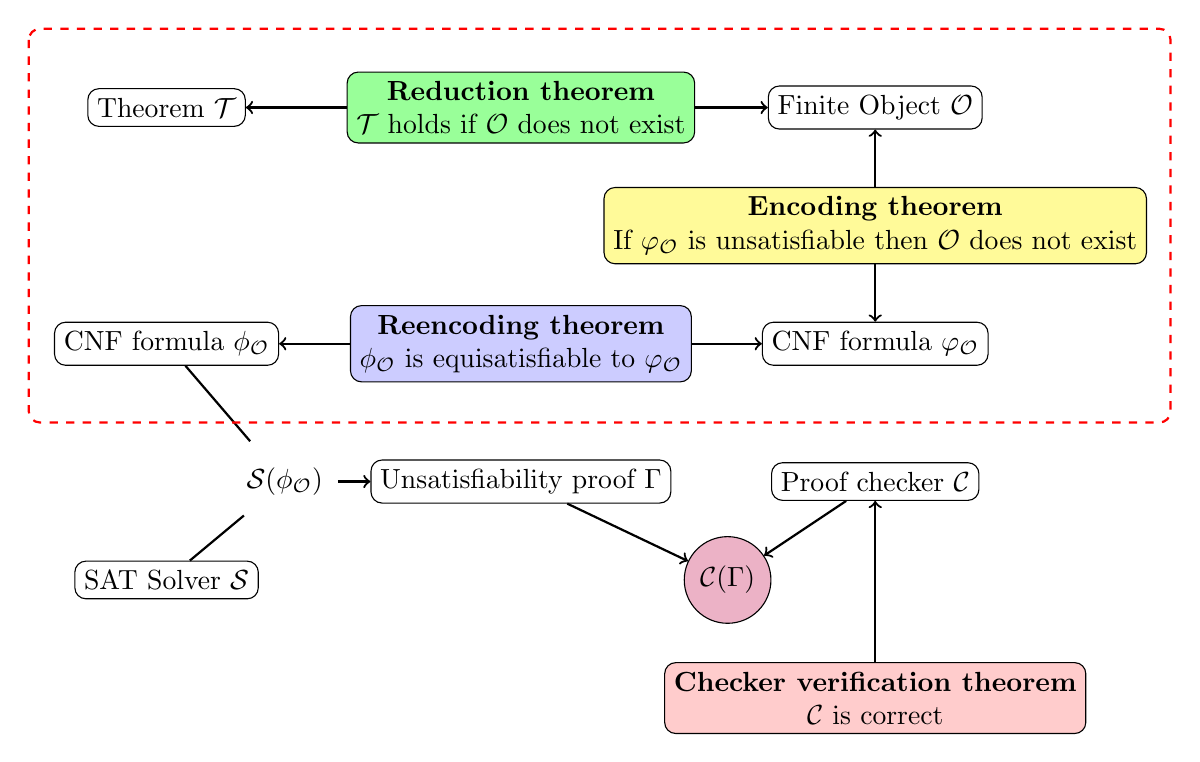
\begin{tikzpicture}
      \node[draw, rounded corners] (theorem) at (0,0) {Theorem $\mathcal{T}$};
      \node[draw, rounded corners] (object) at (9,0) { Finite Object $\mathcal{O}$};
      \node[draw, rounded corners, align=center, fill=green!40!white] (tiffo) at (4.5,0) { \textbf{Reduction theorem}\\$\mathcal{T}$ holds if $\mathcal{O}$ does not exist};
      \draw[->, thick] (tiffo) -- (theorem);
      \draw[->, thick] (tiffo) -- (object);
      \node[draw, rounded corners, align=center] (varphi) at (9, -3) {CNF formula $\varphi_{\mathcal{O}}$};
      \node[draw, rounded corners, align=center, fill=yellow!40!white] (encoding) at (9, -1.5) { \textbf{Encoding theorem}\\If $\varphi_{\mathcal{O}}$ is unsatisfiable then $\mathcal{O}$ does not exist};
      \draw[->, thick] (encoding) -- (object);
      \draw[->, thick] (encoding) -- (varphi);
      \node[draw, rounded corners] (phi) at (0, -3) {CNF formula $\phi_{\mathcal{O}}$};
      \node[draw, rounded corners, align=center, fill=blue!20!white] (equisat) at (4.5, -3) { \textbf{Reencoding theorem}\\$\phi_{\mathcal{O}}$ is equisatisfiable to $\varphi_{\mathcal{O}}$};
      \draw[->, thick] (equisat) -- (phi);
      \draw[->, thick] (equisat) -- (varphi);
      \node[draw, rounded corners] (solver) at (0, -6) {SAT Solver $\mathcal{S}$};
      \node[draw, rounded corners] (unsat-proof) at (4.5, -4.75) {Unsatisfiability proof $\Gamma$};
      \node[circle] (solverphi) at (1.5, -4.75) {$\mathcal{S}(\phi_{\mathcal{O}})$};
      \draw[-, thick] (solver) -- (solverphi);
      \draw[-, thick] (phi) -- (solverphi);
      \draw[->, thick] (solverphi) -- (unsat-proof);
      \node[draw, rounded corners] (checker) at (9, -4.75) {Proof checker $\mathcal{C}$};
      \node[circle, draw, fill=purple!30!white] (checkerphi) at (7.125, -6) {$\mathcal{C}(\Gamma)$};
      \draw[->, thick] (unsat-proof) -- (checkerphi);
      \draw[->, thick] (checker) -- (checkerphi);
      \node[draw, rounded corners, align=center, fill=red!20!white] (checkerCorrectness) at (9, -7.5) { \textbf{Checker verification theorem}\\$\mathcal{C}$ is correct};
  
      \draw[->, thick] (checkerCorrectness) -- (checker);
      \draw[red, dashed, thick, rounded corners] (-1.75,1) -- (-1.75, -4) -- (12.75, -4) -- (12.75, 1) -- cycle;
    \end{tikzpicture}
    \caption{General structure of the verification pipeline for a SAT-based theorem in the \emph{negative case}. The dashed rectangle encloses the main focus of this paper, whereas for the rest of the proof we leverage already existing tools.}\label{fig:proof-structure}
  \end{figure}
The main contribution of this article is to provide the first example of a formally-verified proof of such a theorem in the context of discrete geometry, and the first one overall in Lean, thus addressing different aspects of the question above.
Our proof pipeline involves several components, as illustrated in~\Cref{fig:proof-structure} and described in the rest of the paper.
% \footnote{CC: I'm not sure this characterization is correct. For example, another group of researchers verified in Coq the encoding used in the Pythagorean Triples problem, thus verifying that result. One could say that our contribution is the first \emph{end-to-end} verification, but I don't see how it's inherently distinct from what this other group did with the Pythagorean Triples problem.}

\paragraph{The Empty Hexagon Number.}
In the 1930s, Stein, Erd\H{o}s, and Szekeres mixed geometry and Ramsey theory by studying how many points in the plane in \emph{general position} (i.e., no three points on a common line) are required for a convex $k$-gon to always appear. Let $g(k)$ be the minimum number of points in general position to force a convex $k$-gon.
The celebrated Erd\H{o}s-Szekeres theorem states that $g(k) \leq \binom{2k-4}{k-2} + 1$~\cite{erdosCombinatorialProblemGeometry2009}. Moreover, Erd\H{o}s and Szekeres conjectured that $g(k) = 2^{k-2} + 1$, which has only been proven for $k \leq 6$.

In a similar spirit, Erd\H{o}s defined $h(k)$ as the minimum number of points in general position that is guaranteed to contain a $k$-hole (i.e., a convex $k$-gon without any other point inside).
It is easy to check that $h(3) = 3$ and $h(4) = 5$. In 1978, Harborth established that $h(5) = 10$~\cite{Harborth1978}, and in a surprising turn of events, Horton proved in 1983 that $h(7) = \infty$, meaning one could always avoid $7$-holes~\cite{hortonSetsNoEmpty1983}. 
The only case left open was thus $h(6)$.

The \emph{Empty Hexagon Theorem}, establishing $h(6)$ to be finite, was proven independently by Gerken and Nicolás in 2006, and then refined by Valtr in 2008.
Yet the known range of values for $h(6)$ was quite large, with $29 \leq h(6) \leq 1717$, until Heule and Scheucher used a SAT solver in a recent breakthrough to prove that $h(6) = 30$~\cite{emptyHexagonNumber}, a result we refer to as ``\emph{The Empty Hexagon Number}.''
Now that all the values of $h$ are known, and especially given the extensive computation involved in its proofs, we believe that the final chapter in the story begun by Stein, Erd\H{o}s, and Szekeres is a formal verification of the Empty Hexagon Number.

\paragraph{Related Work.} Despite the crucial role of formal verification in the SAT community (e.g., verified solvers~\cite{oeVersatVerifiedModern2012,skotam_creusat_2022}, proof checking~\cite{lammichEfficientVerifiedSAT2020,tanVerifiedPropagationRedundancy2023}, etc.), the end-to-end formal verification of mathematical proofs obtained through SAT-solving is very recent. To the best of our knowledge, the first and only instance of a formally verified SAT-based mathematical proof before our work corresponds to the Pythagorean Triples Problem, verified in the \textsf{Coq} proof assistant by Cruz-Filipe and Schneider-Kamp~\cite{formalPythagoreanTriples,LPAR-21:Formally_Proving_Boolean_Pythagorean}. In terms of verification of SAT encodings in Lean, the work of Codel, Avigad and Heule pioneered~\cite{Cayden}, while other encoding libraries existed in different frameworks, such as the work of Giljeg\r{a}rd and Wennerbreck in \textsf{CakeML}~\cite{GilAndWennerbeck}, which allowed for verifying SAT-based solutions to different math puzzles (e.g., Sudoku, Kakuro, the \emph{N-queens} problem, etc.).

\paragraph{Outline of the paper.} \Cref{sec:triple-orientations} discusses the basic geometric aspects of the problem, and in particular, \emph{triple orientations} (also known as \emph{signotopes}), a fundamental tool in computational geometry to represent discretely problems involving an a priori continuous space (i.e., $\mathbb{R}^2$), which is the basis of Heule and Scheucher's SAT encoding. Then,~\Cref{sec:symmetry-breaking} deals with two assumptions that are key to break symmetries in the problem and thus make the SAT encoding practically feasible. Namely, that one can assume without loss of generality the following two properties at the same time: (i) points are labeled from left to right without two of them having the same $x$-coordinate, and (ii) the triples $(p_1, p_i, p_j)$ are always oriented counterclockwise for $i < j$. 
\Cref{sec:leansat} presents the \emph{LeanSAT} library, which plays a key role in proving the correctness of encodings. Next,~\Cref{sec:empty-triangle} presents how the previous elements are already enough to formalize a SAT-based proof for the \emph{Empty Triangle Theorem}, a much simpler variant involving only triangles that does not require reencodings. \Cref{sec:empty-hexagon-number} presents the details of the formalization of $h(6) = 30$, the Empty Hexagon Number. We conclude by discussing the next steps towards the formal verification of other Erd\H{o}s-Szekeres-type problems in~\Cref{sec:conclusion}.


\section{Geometric Preliminaries}\label{sec:geometry}
We identify points with elements of $\mathbb{R}^2$. Concretely,~\lstinline|abbrev Point := EuclideanSpace ℝ (Fin 2)|.
The next step is to define what it means for a $k$-gon to be \emph{empty} (with respect to a set of points) and \emph{convex}, which we do in terms of \textsf{mathlib} primitives.

\begin{lstlisting}
/-- `EmptyShapeIn S P' means that `S' carves out an empty shape in `P':
the convex hull of `S' contains no point of `P'
other than those already in `S'. -/
def EmptyShapeIn (S P : Set Point) : Prop :=
    ∀ p ∈ P \ S, p ∉ convexHull ℝ S

/-- `ConvexPoints S' means that `S' consists of extremal points of its convex hull,
i.e. the point set encloses a convex polygon. -/
def ConvexPoints (S : Set Point) : Prop :=
    ∀ a ∈ S, a ∉ convexHull ℝ (S \ {a})

def ConvexEmptyIn (S P : Set Point) : Prop :=
    ConvexPoints S ∧ EmptyShapeIn S P

def HasConvexEmptyKGon (k : Nat) (S : Set Point) : Prop :=
    ∃ s : Finset Point, s.card = k ∧ ↑s ⊆ S ∧ ConvexEmptyIn s S
\end{lstlisting}

Assume for now\footnote{The definition is presented in~\Cref{sec:triple-orientations}.} a predicate \lstinline|ListInGenPos| that states that a list of points is in \emph{general position}, i.e., no three points lie on a common line.
With this we can already state the main theorem of our paper.

\begin{lstlisting}
theorem hole_6_theorem (pts : List Point) (gp : ListInGenPos pts)
    (h : pts.length ≥ 30) : HasConvexEmptyKGon 6 pts.toFinset
\end{lstlisting}

At the root  of the encoding of Heule and Scheucher is the idea that the~\lstinline|ConvexEmptyIn| predicate can be determined by analyzing only triangles. In particular, that a set $s$ of $k$ points in a pointset $S$ form an empty convex $k$-gon if and only if all the ${k \choose 3}$ triangles induced by vertices in $s$ are empty with respect to $S$. This is discussed informally in~\cite[Section 3, Eq.~4]{emptyHexagonNumber}.
Concretely, we prove the following theorem:
\begin{lstlisting}
theorem ConvexEmptyIn.iff_triangles {s : Finset Point} {S : Set Point}
    (sS : ↑s ⊆ S) (sz : 3 ≤ s.card) :
    ConvexEmptyIn s S ↔
    ∀ (t : Finset Point), t.card = 3 → t ⊆ s → ConvexEmptyIn t S
\end{lstlisting}
\begin{figure}
    \centering
    \begin{subfigure}{0.45\textwidth}
        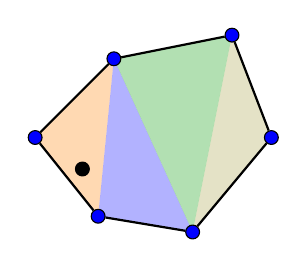
\begin{tikzpicture}
        \coordinate (a) at (0,0);
        \coordinate (b) at (1, 1);
        \coordinate (c) at (2.5, 1.3);
        \coordinate (d) at (3, 0);
        \coordinate (e) at (0.8, -1);
        \coordinate (f) at (2, -1.2);

        \fill[orange, opacity=0.3] (a) -- (b) -- (e) -- (a) -- cycle;
        \fill[blue, opacity=0.3] (b) -- (f) -- (e) -- (b) -- cycle;
        \fill[green!60!black, opacity=0.3] (b) -- (c) -- (f) -- (b) -- cycle;
        \fill[yellow!60!black, opacity=0.3] (c) -- (d) -- (f) -- (c) -- cycle;

        \node[draw, circle, black, fill=blue, inner sep=0pt, minimum size=5pt] (pA) at (0, 0) {};
        \node[draw, circle, black, fill=blue, inner sep=0pt, minimum size=5pt] (pB) at (1, 1) {};
        \node[draw, circle, black, fill=blue, inner sep=0pt, minimum size=5pt] (pC) at (2.5, 1.3) {};
        \node[draw, circle, black, fill=blue, inner sep=0pt, minimum size=5pt] (pD) at (3, 0) {};
        \node[draw, circle, black, fill=blue, inner sep=0pt, minimum size=5pt] (pE) at (0.8, -1) {};
        \node[draw, circle, black, fill=blue, inner sep=0pt, minimum size=5pt] (pF) at (2, -1.2) {};

        \node[draw, circle, black, fill=black, inner sep=0pt, minimum size=5pt] (pG) at (0.6, -0.4) {};


        \draw[thick] (pA) -- (pB) -- (pC) -- (pD) -- (pF) -- (pE) -- (pA);
        % \draw[dashed, thick, red] (pA) -- (pB) -- (pE) -- (pA);
        % \draw[dashed, thick, blue] (pB) -- (pF) -- (pE) -- (pB);
        % \draw[dashed, thick, green!60!black] (pB) -- (pC) -- (pF) -- (pB);


        \end{tikzpicture}
        \caption{}
    \end{subfigure}
    \begin{subfigure}{0.45\textwidth}
        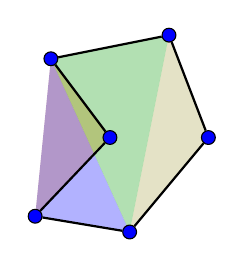
\begin{tikzpicture}
            \coordinate (a) at (1.75,0);
            \coordinate (b) at (1, 1);
            \coordinate (c) at (2.5, 1.3);
            \coordinate (d) at (3, 0);
            \coordinate (e) at (0.8, -1);
            \coordinate (f) at (2, -1.2);

            \fill[orange, opacity=0.3] (a) -- (b) -- (e) -- (a) -- cycle;
            \fill[blue, opacity=0.3] (b) -- (f) -- (e) -- (b) -- cycle;
            \fill[green!60!black, opacity=0.3] (b) -- (c) -- (f) -- (b) -- cycle;
            \fill[yellow!60!black, opacity=0.3] (c) -- (d) -- (f) -- (c) -- cycle;

            \node[draw, circle, black, fill=blue, inner sep=0pt, minimum size=5pt] (pA) at (1.75, 0) {};
            \node[draw, circle, black, fill=blue, inner sep=0pt, minimum size=5pt] (pB) at (1, 1) {};
            \node[draw, circle, black, fill=blue, inner sep=0pt, minimum size=5pt] (pC) at (2.5, 1.3) {};
            \node[draw, circle, black, fill=blue, inner sep=0pt, minimum size=5pt] (pD) at (3, 0) {};
            \node[draw, circle, black, fill=blue, inner sep=0pt, minimum size=5pt] (pE) at (0.8, -1) {};
            \node[draw, circle, black, fill=blue, inner sep=0pt, minimum size=5pt] (pF) at (2, -1.2) {};

            % \node[draw, circle, black, fill=black, inner sep=0pt, minimum size=5pt] (pG) at (0.6, -0.4) {};


            \draw[thick] (pA) -- (pB) -- (pC) -- (pD) -- (pF) -- (pE) -- (pA);
            % \draw[dashed, thick, red] (pA) -- (pB) -- (pE) -- (pA);
            % \draw[dashed, thick, blue] (pB) -- (pF) -- (pE) -- (pB);
            % \draw[dashed, thick, green!60!black] (pB) -- (pC) -- (pF) -- (pB);


        \end{tikzpicture}
        \caption{}
    \end{subfigure}
    \caption{Illustration of the proof for \lstinline|ConvexEmptyIn.iff_triangles|. The left subfigure shows how a point inside the polygon implies the point is inside one of the triangles of triangulation of its convex hull. The right subfigure shows how non-convexity implies one of the vertices of the polygon will be inside one of the triangles of the convex hull partition.}\label{fig:triangulation}
\end{figure}

\begin{proof}[Proof sketch]
    We first prove a simple monotonicity lemma: if $\textsf{ConvexPoints}(s)$, then $\textsf{ConvexPoints}(s')$ for every $s' \subseteq s$, and similarly $\textsf{EmptyShapeIn}(s, S) \Rightarrow \textsf{EmptyShapeIn}(s', S)$ for every set of points $S$.
    By instantiating this monotonicity lemma over all subsets $t \subseteq s$ with $|t| = 3$ we get the forward direction of the theorem.
    For the backward direction it is easier to reason contrapositively: if $s$ does not hold the~$\textsf{ConvexPoints}$ predicate, or is not empty w.r.t.~$S$, then we want to show that there is a triangle $t \subseteq s$ that is also not empty w.r.t.~$S$. To see this, let $H$ be the convex hull of $s$, and then by Carath\'eodory's theorem (cf. \lstinline|theorem convexHull_eq_union| from \textsf{mathlib}), every point in $H$ is a convex combination of at most $3$ points in $s$, and consequently, of exactly $3$ points in $s$.
    If $s$ is non-empty w.r.t.~$S$, then there is a point $p \in S \setminus s$ that belongs to $H$, and by Carath\'eodory, $p$ is a convex combination of $3$ points in $s \setminus \{a\}$, and thus lies inside a triangle $t \subseteq s$ (\Cref{fig:triangulation-a}). If $s$ does not hold $\textsf{ConvexPoints}$, then there is a point $a \in s$ such that $a \in \textsf{convexHull}(s \setminus \{a\})$, and by Carath\'eodory again, $a$ is a convex combination of $3$ points in $s$, and thus lies inside a triangle $t \subseteq s \setminus \{a\}$ (\Cref{fig:triangulation-b}).
%     The
%     The forward direction is easy to see, as triangles are always convex, and if $s$ is empty w.r.t.~$S$, then so are the triangles induced by vertices of $s$.
%     Let $T = \{t_1, \ldots, t_{{k \choose 3}}\}$ be all the triangles induced by vertices of $s$.
%    For the backward direction we will need a \emph{triangulation lemma} stating that the convex hull of $s$ can be partitioned into triangles $P = \{t_i, \ldots, t_j\}$, and $P \subseteq T$.
%     To see that if every $t \in T$ is empty w.r.t. $S$ then $s$ is also empty w.r.t. $S$ we can use the contrapositive statement.
    %  Indeed, assume $s$ is not empty w.r.t. $S$, there is a point $p \in S \setminus s$ that lies inside the convex hull of $s$. Because $P$ is a partition of the convex hull of $s$, point $p$ must be inside some $t \in P \subseteq T$.
    %  To see convexity, we can reason contrapositively again. If $s$ is not convex, then there is a point $p \in s$ that lies inside the convex hull of $s$, and thus lies inside a triangle $t \in P$.
\end{proof}
    
The next section shows how boolean variables can be used to encode which triangles are empty w.r.t.~a pointset, which as the previous theorem shows, can be used to encode the presence or absence of $k$-holes.


\section{Triple Orientations and Base Variables}\label{sec:triple-orientations}
An essential step for obtaining computational proofs of geometric results is \emph{discretization}: problems concerning the existence of an object $\mathcal{O}$ in a continuous space such as $\mathbb{R}^2$ must be reformulated in terms of the existence of a discrete and finitely representable object $\mathcal{O}'$ that a computer can find (or discard its existence).
This poses a particular challenge for problems in which the desired geometric object $\mathcal{O}$ is characterized by very specific coordinates of points, requiring to deal with floating point arithmetic or numerical instability.
Fortunately, this is not the case for Erd\H{o}s-Szekeres-type problems such as determining the value of $h(k)$, which are naturally well-suited for computation.
This is so because the properties of interest (e.g., convexity, emptiness) can be described in terms of high-level relationships between points and lines (e.g., point $p$ is above the line $\vec{qr}$, lines $\vec{qr}$ and $\vec{st}$ intersect, etc.), which are invariant under rotations, translations, and even small perturbations of the coordinates. This suggests the problems can be discretized in terms of boolean variables representing these high-level relationships, forgetting the specific coordinates of the points.
The combinatorial abstraction that has been most widely used in Erd\H{o}s-Szekeres-type problems is that of \emph{triple orientations}~\cite{ emptyHexagonNumber, scheucherTwoDisjoint5holes2020}.\footnote{Also known as \emph{signotopes}~\cite{felsnerSweepsArrangementsSignotopes2001,subercaseaux2023minimizing},  Knuth's \emph{counterclockwise} relation~\cite{knuthAxiomsHulls1992}, or \emph{signatures}~\cite{szekeres_peters_2006}.}
Given points $p, q, r$, their \emph{triple-orientation} is defined as
\newcommand{\sign}{\operatorname{sign}}
\[
  \sigma(p, q, r) = \sign \det \begin{pmatrix} p_x & q_x & r_x \\ p_y & q_y & r_y \\ 1 & 1 & 1 \end{pmatrix} = \begin{cases}
    1 & \text{if } p, q, r \text{ are \emph{oriented} counterclockwise}, \\
    0 & \text{if } p, q, r \text{ are collinear}, \\
    -1 & \text{if } p, q, r \text{ are \emph{oriented} clockwise}.
  \end{cases}.
\]

\begin{figure}
  \centering
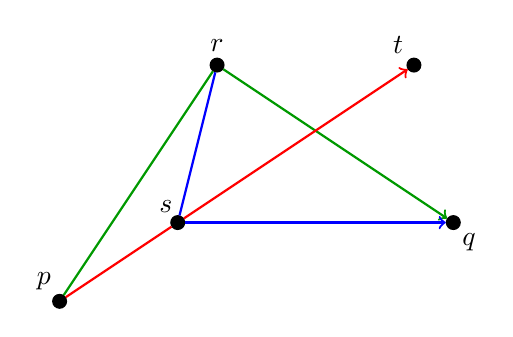
\begin{tikzpicture}
  %\draw[ultra thick, dashed, blue] (5,1) -- (0,0);
  \node[draw, circle, black, fill=black, inner sep=0pt, minimum size=5pt] (p) at (0,0) {};
  \node[] at (-0.2, 0.25) {$p$};
  \node[draw, circle, black, fill=black, inner sep=0pt, minimum size=5pt] (q) at (5,1) {};
  \node[] at (5.2, 0.75) {$q$};
  \node[draw, circle, black, fill=black, inner sep=0pt, minimum size=5pt] (r) at (2,3) {};
  \node[] at (2, 3.25) {$r$};

  \node[draw, circle, black, fill=black, inner sep=0pt, minimum size=5pt] (s) at (1.5, 1) {};
  \node[] at (1.35, 1.2) {$s$};

  \node[draw, circle, black, fill=black, inner sep=0pt, minimum size=5pt] (t) at (4.5, 3) {};
  \node[] at (4.3, 3.25) {$t$};

  \draw[ thick,  green!60!black] (p) -- (r);
  \draw[ thick,  green!60!black, ->] (r) -- (q);

  \draw[ thick,  blue] (r) -- (s);
  \draw[ thick,  blue, ->] (s) -- (q);

  \draw[thick,  red] (p) -- (s);
  \draw[thick,  red, ->] (s) -- (t);
  % \draw[fill=green, opacity=0.5] (a.center) -- (b.center) -- (c.center) -- cycle;
\end{tikzpicture}
\caption{Illustration of triple orientations, where $\sigma(p, r, q) = -1, \sigma(r, s, q) = 1, $ and $\sigma(p, s, t) = 0$.}\label{fig:triple-orientation}
\end{figure}

An example is illustrated in~\Cref{fig:triple-orientation}. Formally, we identify points with members of $\mathbb{R}^2$, and use \textsf{mathlib}'s definition of the determinant to define $\sigma$.
% @[pp_dot] abbrev x (p : Point) : ℝ := p 0
% @[pp_dot] abbrev y (p : Point) : ℝ := p 1
\begin{lstlisting}
abbrev Point := EuclideanSpace ℝ (Fin 2)

inductive Orientation : Type where
  | cw -- clockwise :=  -
  | ccw -- counter clockwise := +
  | collinear -- := 0

noncomputable def σ (p q r : Point) : Orientation :=
  let det := Matrix.det !![p.x, q.x, r.x ; p.y, q.y, r.y ; 1, 1, 1]
  if 0 < det then ccw
  else if det < 0 then cw
  else collinear
\end{lstlisting}

% def Orientation.ofReal (r : ℝ) : Orientation :=
%   if 0 < r then ccw
%   else if r < 0 then cw
%   else collinear

Through the $\sigma$ function we can immediately define the notion of \emph{general position} for collections (e.g., finite sets, lists, etc.) of points, simply establishing that $\sigma(p, q, r) \neq 0$ for every three distinct points $p, q, r$ in the collection.
Furthermore, we can start formalizing sets of points that are \emph{equivalent} with respect to their triple orientations, and consequently, properties of pointsets that are fully captured by their triple orientations~(\emph{orientation properties}). 
% An illustration is presented in~\Cref{fig:sigma-equiv}.
% \begin{figure}
    \centering
    \begin{subfigure}{0.3\linewidth}
        \centering
        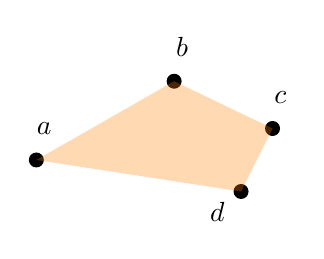
\begin{tikzpicture}
            \node[draw, circle, black, fill=black, inner sep=0pt, minimum size=5pt, label={[xshift=0.1cm, yshift=0.1cm]$a$}] (a) at (0,0) {};
            \node[draw, circle, black, fill=black, inner sep=0pt, minimum size=5pt, label={[xshift=0.1cm, yshift=0.1cm]$b$}] (b) at (1.75,1) {};
            \node[draw, circle, black, fill=black, inner sep=0pt, minimum size=5pt, label={[xshift=0.1cm, yshift=0.1cm]$c$}] (c) at (3,0.4) {};
            \node[draw, circle, black, fill=black, inner sep=0pt, minimum size=5pt, label={[xshift=-0.3cm, yshift=-0.6cm]$d$}] (d) at (2.6,-0.4) {};
            \coordinate (a) at (0,0);
            \coordinate (b) at (1.75,1);
            \coordinate (c) at (3,0.4);
            \coordinate (d) at (2.6,-0.4);
            \fill[orange, opacity=0.3] (a) -- (b) -- (c) -- (d) -- (a) -- cycle;
        \end{tikzpicture}
        \caption{The signature induced by $\sigma$ is $\texttt{-\,-\,-\,-}$.}
    \end{subfigure}
    \begin{subfigure}{0.3\linewidth}
        \centering
        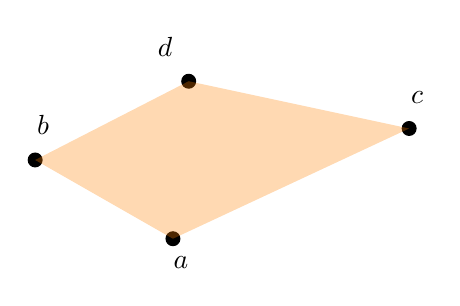
\begin{tikzpicture}
            \node[draw, circle, black, fill=black, inner sep=0pt, minimum size=5pt, label={[xshift=0.1cm, yshift=-0.6cm]$a$}] (a) at (0,0) {};
            \node[draw, circle, black, fill=black, inner sep=0pt, minimum size=5pt, label={[xshift=0.1cm, yshift=0.1cm]$b$}] (b) at (-1.75,1) {};
            \node[draw, circle, black, fill=black, inner sep=0pt, minimum size=5pt, label={[xshift=0.1cm, yshift=0.1cm]$c$}] (c) at (3,1.4) {};
            \node[draw, circle, black, fill=black, inner sep=0pt, minimum size=5pt, label={[xshift=-0.3cm, yshift=0.1cm]$d$}] (d) at (0.2,2) {};
            \coordinate (a) at (0,0);
            \coordinate (b) at (-1.75,1);
            \coordinate (c) at (3,1.4);
            \coordinate (d) at (0.2,2);
            \fill[orange, opacity=0.3] (b) -- (d) -- (c) -- (a) -- (b) -- cycle;
        \end{tikzpicture}
        \caption{The signature induced by $\sigma$ is $\texttt{-\,-\,+\,-}$.}
    \end{subfigure}
    \begin{subfigure}{0.3\linewidth}
        \centering
        
\begin{tikzpicture}
            \node[draw, circle, black, fill=black, inner sep=0pt, minimum size=5pt] (p) at (0,0) {};
        \end{tikzpicture}
    \end{subfigure}
  \caption{Illustration of the notion of $\sigma$-equivalence.}\label{fig:sigma-equiv}
  \end{figure}

\begin{lstlisting}
  structure σEquiv (S T : Set Point) where
    f : Point → Point
    bij : Set.BijOn f S T 
    parity : Bool -- See Section 4 for a more detialed explanation 
    σ_eq : ∀ (p ∈ S) (q ∈ S) (r ∈ S), σ p q r = parity ^^^ σ (f p) (f q) (f r)
    
  def OrientationProperty (P : List Point → Prop) :=
    ∀ {{S T}}, S ≃σ T → (P S ↔ P T) -- `≃σ` is infix notation for `σEquiv`
\end{lstlisting}

For an initial example of how these notions will be used, let us consider the property
\[
  \pi(P) \triangleq \text{\em ``pointset P contains an empty triangle''}.
\]

We start by relating a \textsf{mathlib}-like definition of what it means for a point $a$ to be inside a triangle $pqr$ with a definition based on triple orientations. As we prove the property can be defined in terms of triple orientations, we obtain as a result that $\pi$ is an orientation property.

\begin{lstlisting}
def PtInTriangle (a p q r : Point) : Prop := a ∈ convexHull ℝ {p, q, r}

def σPtInTriangle (a p q r : Point) : Prop :=
  σ p q r = σ p a r ∧ σ p a q = σ p r q ∧ σ q a r = σ q p r

theorem σPtInTriangle_iff {a p q r : Point} (gp : PtFinsetInGenPos {a,p,q,r}) :
  σPtInTriangle a p q r ↔ PtInTriangle a p q r -- not trivial.

def HasEmptyTriangle (pts : Set Point) : Prop := ∃ p q r, [p, q, r].Nodup
∧ {p,q,r} ⊆ pts ∧ ∀ a ∈ pts, a ∉ ({p, q, r} : Set Point) → ¬PtInTriangle a p q r

theorem OrientationProperty_HasEmptyTriangle : OrientationProperty HasEmptyTriangle
\end{lstlisting}

Let us now discuss the previous steps. First,~\lstinline|(PtInTriangle a p q r)| presents a \emph{ground-truth}  definition for membership in a triangle, in terms of~\textsf{mathlib}'s \lstinline|ConvexHull| definition,  whereas~\lstinline|(σPtInTriangle a p q r)| is based on orientations. Heule and Scheucher used the orientation-based definition~\cite{emptyHexagonNumber}, and as it is common in the area, its equivalence to the \emph{ground-truth} mathematical definition was left implicit. This equivalnce, proven in~\lstinline|theorem σPtInTriangle_iff| is not obvious. Next, we have proved that ``having an empty triangle'' is an orientation property, but \textbf{why is that relevant?} Let us highlight two reasons for why this definition of orientation properties plays an important role in the formalization of Erd\H{o}s-Szekeres-type problems:
\begin{enumerate}
  \item If we prove that the function $\sigma$ is invariant under a certain transformation of its arguments (e.g., rotations, translations, etc.) then we can directly conclude that any orientation property is invariant under the same transformation. This is a powerful tool for applying manipulations to pointsets that preserve the properties of interest, which will be key for symmetry breaking (see~\Cref{sec:symmetry-breaking}). For a concrete example, when a proof for an Erd\H{o}s-Szekeres-type result starts saying \emph{``we assume without loss of generality that points $p_1, \ldots, p_n$ are sorted from left to right''}, we can immediately formalize that this assumption indeed maintains generality for orientation properties, as sorting a list naturally induces a bijection.
  \item As introduced at the beginning of this section, SAT encodings for Erd\H{o}s-Szekeres-type problems are based on capturing properties like convexity or emptiness in terms of triple orientations, thus reducing a continuous search space to a discrete one. The fact that for a certain property $\pi$ we can search over the space of triple orientations instead of $\mathbb{R}^2$ is precisely what the definiton of \emph{orientation property} captures. In other words, this is the key idea that will allow us to transition from the finitely-verifiable statement \emph{``no set of triple orientations over $n$ points satisfies property $\pi$''} to \emph{``no set of $n$ points satisfies property $\pi$''}.
\end{enumerate}



\subsection{Some key properties of the $\sigma$ function}
A few properties of the $\sigma$ function are heavily used in SAT encodings, ranging from the initial work of Peters and Szekeres~\cite{szekeres_peters_2006} to the recent work of Heule and Scheucher~\cite{emptyHexagonNumber}. At the base of such encodings, boolean variables $\orvar_{p,q,r}$ are used to represent $\sigma(p, q, r) = 1$\footnote{Given that pointsets are assumed to be in general position we have $\neg \orvar_{p,q,r} \iff \sigma(p, q, r) = -1$.}. If one were to create a variable $\orvar_{p,q,r}$ for every triple of points $p \neq q \neq r$, that would amount to $n(n-1)(n-2)$ variables for $n$ points. However, the orientations of triples $(p, q, r)$ and $(q, r, p)$ or $(r, q, p)$ contain redundant information: if $p,q,r$ are oriented counterclockwise, then $q,r,p$ and $r,p,q$ are also oriented counterclockwise, whereas $p,r,q$ is oriented clockwise. This is captured by the following two fundamental asymmetries:
\begin{lstlisting}
  theorem σ_perm₁ (p q r : Point) : σ p q r = -σ q p r
  theorem σ_perm₂ (p q r : Point) : σ p q r = -σ p r q
\end{lstlisting}
As a result, the number of boolean variables needed for the SAT encoding can be reduced by a factor of $3! = 6$.

Now, consider four points $p, q, r, s$ that are sorted from left to right. If $p, q, r$ are oriented counterclockwise, and $q, r, s$ are oriented counterclockwise as well, then it follows that $p, r, s$ must be oriented counterclockwise too (see~\Cref{fig:orientation-implication}). Different \emph{$\sigma$-implication-properties} of this form are used to reduce the search space in SAT encodings~\cite{emptyHexagonNumber,scheucherTwoDisjoint5holes2020,subercaseaux2023minimizing, szekeres_peters_2006}, as they can be easily added in clausal form:
\begin{align}
  &\left(\neg \orvar_{p, q, r} \lor \neg \orvar_{p, r, t} \lor \orvar_{p, q, t}\right) \land \left(\orvar_{p, q, r} \lor \orvar_{p, r, t} \lor  \neg \orvar_{p, q, t}\right), \\
  &\left(\neg \orvar_{p, q, r} \lor \neg \orvar_{q, r, t} \lor  \orvar_{p, r, t}\right) \land \left(\orvar_{p, q, r} \lor \orvar_{q, r, t} \lor  \neg \orvar_{p, r, t}\right).
\end{align}

We formalize these implication properties and prove their validity, as for example:
\begin{lstlisting}
theorem σ_prop₁ {p q r s : Point} (h : Sorted₄ p q r s) (hGp : InGenPos₄ p q r s) :
    σ p q r = ccw → σ q r s = ccw → σ p r s = ccw
\end{lstlisting}

% [...]

% theorem σ_prop₃ {p q r s : Point} (h : Sorted₄ p q r s) (hGp : InGeneralPosition₄ p q r s) :
%     σ p q r = cw → σ q r s = cw → σ p r s = cw
The proofs of these properties are based on an equivalence between the orientation of a triple of points and the \emph{slopes} of the lines that connect them. Namely, if $p, q, r$  are sorted from left to right, then (i) $\sigma(p,q,r)=1 \iff \textsf{slope}(\vec{pq}) < \textsf{slope}(\vec{pr})$  and (ii) $\sigma(p,q,r)=1 \iff \textsf{slope}(\vec{pr}) < \textsf{slope}(\vec{qr})$. By proving first these \emph{slope-orientation} equivalences we can then easily prove e.g.,~\lstinline|σ_prop₁|, as illustrated in~\Cref{fig:orientation-implication}.

\begin{figure}
  \centering
  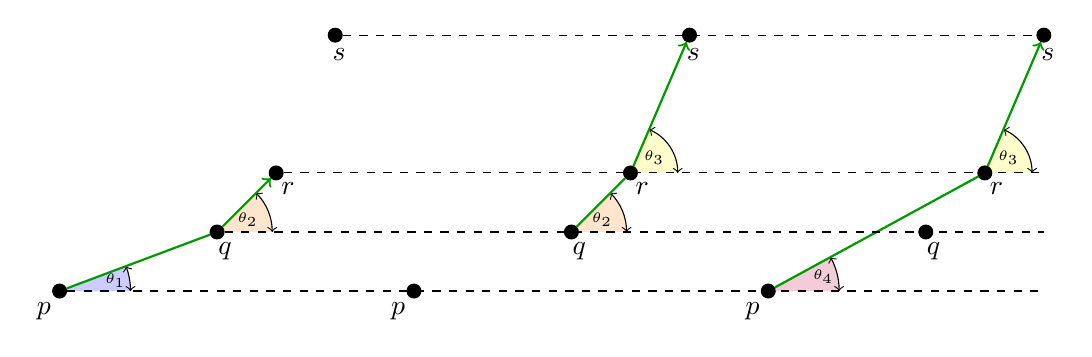
\begin{tikzpicture}
    \newcommand{\localspacing}{4.5}

    \foreach \i in {0, 1, 2} {

      \coordinate (p\i) at ( \i*\localspacing +0.5,0);
      \coordinate (q\i) at ( \i*\localspacing +2.5, 0.75);
      \coordinate (r\i) at ( \i*\localspacing +3.25, 1.5);
      \coordinate (s\i) at ( \i*\localspacing +4.0, 3.25);
    }
    \coordinate (0p) at (13,0);
    \coordinate (0q) at (13, 0.75);
    \coordinate (0r) at (13, 1.5);
    \coordinate (0s) at (13, 3.25);

    \pic [draw, <->,
    angle radius=9mm, angle eccentricity=0.8, fill=blue!20!white,
    "$\text{\tiny{\(\theta_1\)}}$"] {angle = 0p--p0--q0};

    \pic [draw, <->,
    angle radius=7mm, angle eccentricity=0.6, fill=orange!20!white,
    "$\text{\tiny{\(\theta_2\)}}$"] {angle = 0q--q0--r0};


    \pic [draw, <->,
    angle radius=7mm, angle eccentricity=0.6, fill=orange!20!white,
    "$\text{\tiny{\(\theta_2\)}}$"] {angle = 0q--q1--r1};

    \pic [draw, <->,
    angle radius=6mm, angle eccentricity=0.6, fill=yellow!20!white,
    "$\text{\tiny{\(\theta_3\)}}$"] {angle = 0r--r1--s1};


    \pic [draw, <->,
    angle radius=9mm, angle eccentricity=0.8, fill=purple!20!white,
    "$\text{\tiny{\(\theta_4\)}}$"] {angle = 0p--p2--r2};


    \pic [draw, <->,
    angle radius=6mm, angle eccentricity=0.6, fill=yellow!20!white,
    "$\text{\tiny{\(\theta_3\)}}$"] {angle = 0r--r2--s2};



    \foreach \i in {0, 1, 2} {

      \node[draw, circle, black, fill=black, inner sep=0pt, minimum size=5pt] (p\i) at ( \i*\localspacing +0.5,0) {};
      \node[] at ( \i*\localspacing + 0.3, -0.25) {$p$};
      \node[draw, circle, black, fill=black, inner sep=0pt, minimum size=5pt] (q\i) at ( \i*\localspacing +2.5, 0.75) {};
      \node[] at ( \i*\localspacing +2.6, 0.5) {$q$};
      \node[draw, circle, black, fill=black, inner sep=0pt, minimum size=5pt] (r\i) at ( \i*\localspacing +3.25, 1.5) {};
      \node[] at ( \i*\localspacing +3.4, 1.3) {$r$};

      \node[draw, circle, black, fill=black, inner sep=0pt, minimum size=5pt] (s\i) at ( \i*\localspacing +4.0, 3.25) {};
      \node[] at ( \i*\localspacing +4.05, 3) {$s$};
    }

    % \newcommand{\localdx}{0.25}
    % \newcommand{\localdy}{-0.5}
    \draw[thick, green!60!black] (p0) -- (q0);
    \draw[thick, green!60!black, ->] (q0) -- (r0);

    \draw[ thick, green!60!black] (q1) -- (r1);
    \draw[ thick, green!60!black, ->] (r1) -- (s1);

    \draw[ thick, green!60!black] (p2) -- (r2);
    \draw[ thick, green!60!black, ->] (r2) -- (s2);
    % \draw[  dashed, green!60!black] (0 + \localdx, 0 + \localdy) -- (2.5 + \localdx, 0.75 + \localdy);
    % \draw[ dashed, green!60!black, ->] (2.5 + \localdx, 0.75 + \localdy) -- (3.25 + \localdx, 1.5 + \localdy);


    % \draw[  dashed, green!60!black] (2.5  - \localdx, 0.75 - \localdy) -- (3.25 - \localdx, 1.5 - \localdy);
    % \draw[ dashed, green!60!black, ->] (3.25 - \localdx, 1.5 - \localdy) -- (4.25  - \localdx, 3.25 - \localdy);

    % \draw[ thick, dashed, green!60!black] (p) -- (r);
    % \draw[ thick, dashed, green!60!black, ->] (r) -- (s);


    \draw[dashed] (p0) -- (0p);
    \draw[dashed] (q0) -- (0q);
    \draw[dashed] (r0) -- (0r);
    \draw[dashed] (s0) -- (0s);



  \end{tikzpicture}
  \caption{Illustration for $\sigma(p,q,r) = 1 \; \land \; \sigma(q,r,s) = 1 \implies \sigma(p, r, s) = 1$. As we have assumptions $\theta_3 > \theta_2 > \theta_4$  by the forward direction of the \emph{slope-orientation equivalence}, we deduce $\theta_3 > \theta_4$, and then conclude $\sigma(p, r, s) = 1$ by the backward direction of the \emph{slope-orientation equivalence}.  }\label{fig:orientation-implication}
\end{figure}


\section{Properties of $\sigma$}\label{sec:properties-of-sigma}
We now prove that, assuming points will be sorted left to right (which is justified in~\Cref{sec:symmetry-breaking}), then the clauses in~\Cref{eq:constraint-4,eq:constraint-5} are justified.
Consider four points $p, q, r, s$ that are sorted from left to right. If $p, q, r$ are oriented counterclockwise, and $q, r, s$ are oriented counterclockwise as well, then it follows that $p, r, s$ must be oriented counterclockwise too (see~\Cref{fig:orientation-implication}). Different \emph{$\sigma$-implication-properties} of this form are used to reduce the search space in SAT encodings~\cite{emptyHexagonNumber,scheucherTwoDisjoint5holes2020,subercaseaux2023minimizing, szekeres_peters_2006}, as they can be easily added in clausal form:
\begin{align}
  &\left(\neg \orvar_{a, b, c} \lor \neg \orvar_{a, c, d} \lor \orvar_{a, b, d}\right) \land \left(\orvar_{a, b, c} \lor \orvar_{a, c, d} \lor  \neg \orvar_{a, b, d}\right)
\end{align}

We prove these properties of the $\sigma$ function, justifying the addition of~\Cref{eq:constraint-4,eq:constraint-5}, as well as other similar properties that are useful for other proofs, even if not explicitly added to the encoding.
\begin{lstlisting}
theorem σ_prop₁ {p q r s : Point} (h : Sorted₄ p q r s) (hGp : InGenPos₄ p q r s) :
    σ p q r = ccw → σ q r s = ccw → σ p r s = ccw

 [...]

theorem σ_prop₃ {p q r s : Point} (h : Sorted₄ p q r s) (hGp : InGeneralPosition₄ p q r s) :
    σ p q r = cw → σ q r s = cw → σ p r s = cw
\end{lstlisting}


The proofs of these properties are based on an equivalence between the orientation of a triple of points and the \emph{slopes} of the lines that connect them. Namely, if $p, q, r$  are sorted from left to right, then (i) $\sigma(p,q,r)=1 \iff \textsf{slope}(\vec{pq}) < \textsf{slope}(\vec{pr})$  and (ii) $\sigma(p,q,r)=1 \iff \textsf{slope}(\vec{pr}) < \textsf{slope}(\vec{qr})$. By proving first these \emph{slope-orientation} equivalences we can then easily prove e.g.,~\lstinline|σ_prop₁|, as illustrated in~\Cref{fig:orientation-implication}.

\begin{figure}
  \centering
  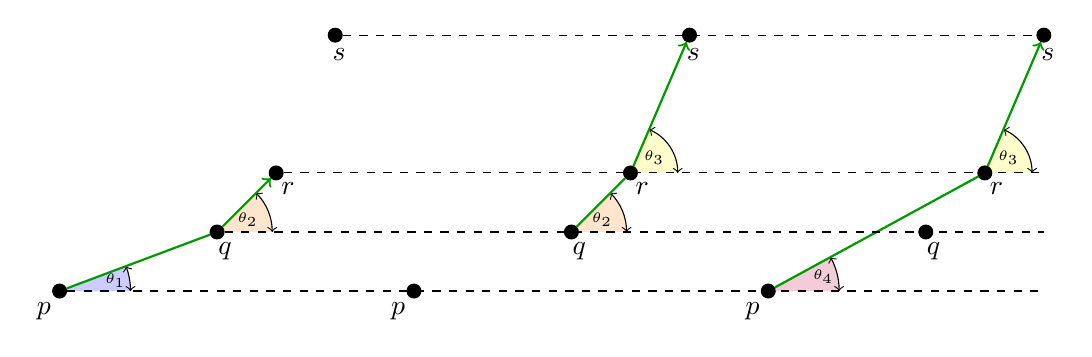
\begin{tikzpicture}
    \newcommand{\localspacing}{4.5}

    \foreach \i in {0, 1, 2} {

      \coordinate (p\i) at ( \i*\localspacing +0.5,0);
      \coordinate (q\i) at ( \i*\localspacing +2.5, 0.75);
      \coordinate (r\i) at ( \i*\localspacing +3.25, 1.5);
      \coordinate (s\i) at ( \i*\localspacing +4.0, 3.25);
    }
    \coordinate (0p) at (13,0);
    \coordinate (0q) at (13, 0.75);
    \coordinate (0r) at (13, 1.5);
    \coordinate (0s) at (13, 3.25);

    \pic [draw, <->,
    angle radius=9mm, angle eccentricity=0.8, fill=blue!20!white,
    "$\text{\tiny{\(\theta_1\)}}$"] {angle = 0p--p0--q0};

    \pic [draw, <->,
    angle radius=7mm, angle eccentricity=0.6, fill=orange!20!white,
    "$\text{\tiny{\(\theta_2\)}}$"] {angle = 0q--q0--r0};


    \pic [draw, <->,
    angle radius=7mm, angle eccentricity=0.6, fill=orange!20!white,
    "$\text{\tiny{\(\theta_2\)}}$"] {angle = 0q--q1--r1};

    \pic [draw, <->,
    angle radius=6mm, angle eccentricity=0.6, fill=yellow!20!white,
    "$\text{\tiny{\(\theta_3\)}}$"] {angle = 0r--r1--s1};


    \pic [draw, <->,
    angle radius=9mm, angle eccentricity=0.8, fill=purple!20!white,
    "$\text{\tiny{\(\theta_4\)}}$"] {angle = 0p--p2--r2};


    \pic [draw, <->,
    angle radius=6mm, angle eccentricity=0.6, fill=yellow!20!white,
    "$\text{\tiny{\(\theta_3\)}}$"] {angle = 0r--r2--s2};



    \foreach \i in {0, 1, 2} {

      \node[draw, circle, black, fill=black, inner sep=0pt, minimum size=5pt] (p\i) at ( \i*\localspacing +0.5,0) {};
      \node[] at ( \i*\localspacing + 0.3, -0.25) {$p$};
      \node[draw, circle, black, fill=black, inner sep=0pt, minimum size=5pt] (q\i) at ( \i*\localspacing +2.5, 0.75) {};
      \node[] at ( \i*\localspacing +2.6, 0.5) {$q$};
      \node[draw, circle, black, fill=black, inner sep=0pt, minimum size=5pt] (r\i) at ( \i*\localspacing +3.25, 1.5) {};
      \node[] at ( \i*\localspacing +3.4, 1.3) {$r$};

      \node[draw, circle, black, fill=black, inner sep=0pt, minimum size=5pt] (s\i) at ( \i*\localspacing +4.0, 3.25) {};
      \node[] at ( \i*\localspacing +4.05, 3) {$s$};
    }

    % \newcommand{\localdx}{0.25}
    % \newcommand{\localdy}{-0.5}
    \draw[thick, green!60!black] (p0) -- (q0);
    \draw[thick, green!60!black, ->] (q0) -- (r0);

    \draw[ thick, green!60!black] (q1) -- (r1);
    \draw[ thick, green!60!black, ->] (r1) -- (s1);

    \draw[ thick, green!60!black] (p2) -- (r2);
    \draw[ thick, green!60!black, ->] (r2) -- (s2);
    % \draw[  dashed, green!60!black] (0 + \localdx, 0 + \localdy) -- (2.5 + \localdx, 0.75 + \localdy);
    % \draw[ dashed, green!60!black, ->] (2.5 + \localdx, 0.75 + \localdy) -- (3.25 + \localdx, 1.5 + \localdy);


    % \draw[  dashed, green!60!black] (2.5  - \localdx, 0.75 - \localdy) -- (3.25 - \localdx, 1.5 - \localdy);
    % \draw[ dashed, green!60!black, ->] (3.25 - \localdx, 1.5 - \localdy) -- (4.25  - \localdx, 3.25 - \localdy);

    % \draw[ thick, dashed, green!60!black] (p) -- (r);
    % \draw[ thick, dashed, green!60!black, ->] (r) -- (s);


    \draw[dashed] (p0) -- (0p);
    \draw[dashed] (q0) -- (0q);
    \draw[dashed] (r0) -- (0r);
    \draw[dashed] (s0) -- (0s);



  \end{tikzpicture}
  \caption{Illustration for $\sigma(p,q,r) = 1 \; \land \; \sigma(q,r,s) = 1 \implies \sigma(p, r, s) = 1$. As we have assumptions $\theta_3 > \theta_2 > \theta_4$  by the forward direction of the \emph{slope-orientation equivalence}, we deduce $\theta_3 > \theta_4$, and then conclude $\sigma(p, r, s) = 1$ by the backward direction of the \emph{slope-orientation equivalence}.  }\label{fig:orientation-implication}
\end{figure}


% \section{The Empty Triangle Theorem}\label{sec:empty-triangle}
% Let us consider a much simpler theorem, which we call the \emph{empty triangle theorem}. Its proof will be helpful to motivate the different aspects of our formalization of the empty hexagon theorem.

\begin{theorem}[Empty Triangle Theorem]
  \label{thm:empty-triangle}
  Given a set $S$ of $n \geq 3$ points in general position, there exists $3$ points $a, b, c \in S$ such that no point $d \in S$ lies inside the triangle $abc$.
\end{theorem}

\begin{proof}[(Human Proof)]
    Let $a, b, x$ be any three points of $S$.
    Define the relation $p \prec q$ to mean that the triangle $abp$ is contained inside the triangle $abq$. Note that $\prec$ is a finite partial order, and thus there must exist at least one minimal element for $\prec$.
    Let $c$ be a minimal element of $\prec$, and now note that $abc$ cannot contain any other point $d \in  S$, as otherwise we would have $d \prec c$, contradicting the minimality of $c$. An illustration of this proof is presented in~\Cref{fig:empty-triangle}.
\end{proof}

\begin{figure}
\centering
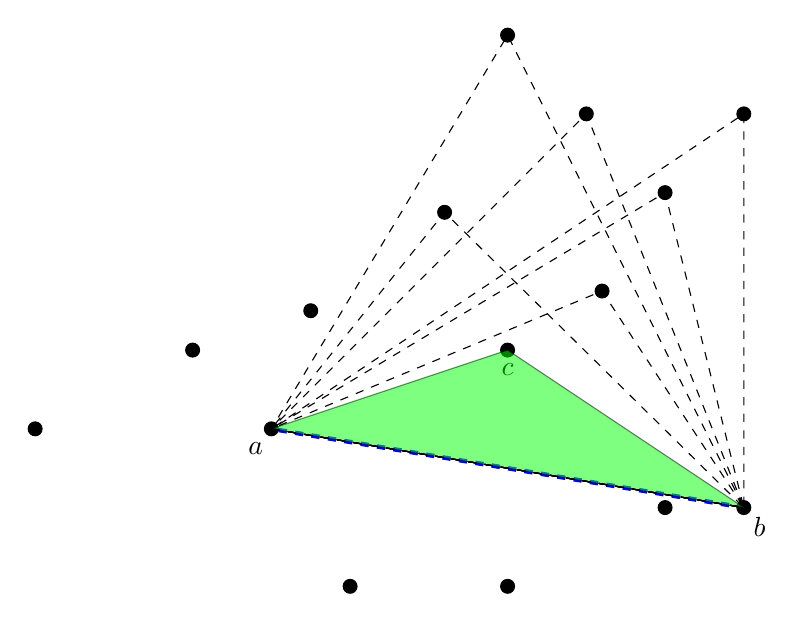
\begin{tikzpicture}
\node[draw, circle, black, fill=black, inner sep=0pt, minimum size=5pt] (h) at (0,0) {};
\node[draw, circle, black, fill=black, inner sep=0pt, minimum size=5pt] (c) at (2,3) {};
\node[] at (2, 2.75) {$c$};
\node[draw, circle, black, fill=black, inner sep=0pt, minimum size=5pt] (p) at (1.2,4.75) {};
\node[draw, circle, black, fill=black, inner sep=0pt, minimum size=5pt] (d) at (4,1) {};
\node[draw, circle, black, fill=black, inner sep=0pt, minimum size=5pt] (e) at (5,6) {};
\node[draw, circle, black, fill=black, inner sep=0pt, minimum size=5pt] (f) at (2,7) {};
\node[draw, circle, black, fill=black, inner sep=0pt, minimum size=5pt] (g) at (4,5) {};
\node[draw, circle, black, fill=black, inner sep=0pt, minimum size=5pt] (a) at (-1,2) {};
\node[] at (-1.2, 1.75) {$a$};
\node[draw, circle, black, fill=black, inner sep=0pt, minimum size=5pt] (i) at (-2,3) {};
\node[draw, circle, black, fill=black, inner sep=0pt, minimum size=5pt] (j) at (-0.5, 3.5) {};
% \node[draw, circle, black, fill=black, inner sep=0pt, minimum size=5pt] (k) at (2.5,-1) {};
\node[draw, circle, black, fill=black, inner sep=0pt, minimum size=5pt] (l) at (3,6) {};
\node[draw, circle, black, fill=black, inner sep=0pt, minimum size=5pt] (m) at (-4,2) {};
% \node[draw, circle, black, fill=black, inner sep=0pt, minimum size=5pt] (n) at (-2, -2) {};
\node[draw, circle, black, fill=black, inner sep=0pt, minimum size=5pt] (o) at (2, 0) {};

\node[draw, circle, black, fill=black, inner sep=0pt, minimum size=5pt] (b) at (5,1) {};
\node[] at (5.2, 0.75) {$b$};

\node[draw, circle, black, fill=black, inner sep=0pt, minimum size=5pt] (q) at (3.2, 3.75) {};

\draw[ultra thick, dashed, blue] (a) -- (b);
\draw[fill=green, opacity=0.5] (a.center) -- (b.center) -- (c.center) -- cycle;
\draw[dashed] (a.center) -- (b.center) -- (l.center) -- cycle;
\draw[dashed] (a.center) -- (b.center) -- (g.center) -- cycle;
\draw[dashed] (a.center) -- (b.center) -- (e.center) -- cycle;
\draw[dashed] (a.center) -- (b.center) -- (q.center) -- cycle;
\draw[dashed] (a.center) -- (b.center) -- (f.center) -- cycle;
\draw[dashed] (a.center) -- (b.center) -- (p.center) -- cycle;

\end{tikzpicture}
\caption{An illustration of the proof for~\Cref{thm:empty-triangle}.}
\label{fig:empty-triangle}
\end{figure}

Instead of formalizing the above proof, we will formalize a SAT-based proof, with the goal of approaching the formalization of the empty hexagon theorem.
Naturally, to use a  SAT-solver we need to parameterize~\Cref{thm:empty-triangle} by $n = |S|$, the number of points, and generate a different proof for each value of $n \geq 3$. For example, consider the following theorem.

\begin{lstlisting}
  theorem EmptyTriangle10Theorem (pts : Finset Point)
    (gp : PointFinsetInGeneralPosition pts)
    (h : pts.card = 10) :
    ∃ (p q r : Point), {p, q, r} ⊆ pts ∧ EmptyTriangleIn p q r pts
\end{lstlisting}

To complete the statement of the theorem, we must define~\texttt{EmptyTriangleIn}, and before that what it means for a point to be \emph{inside} a triangle.

\begin{lstlisting}
  def pt_in_triangle (a : Point) (p q r : Point) : Prop :=
    ∃ p' q' r', ({p', q', r'} : Set Point) = {p, q, r} ∧
      Sorted₃ p' q' r' ∧
      Sorted₃ p' a r' ∧
      a ≠ q' ∧ -- this isn't needed if p,q,r are in GP
      σ p' q' r' = σ p' a r' ∧
      σ p' a q' = σ p' r' q' ∧
      σ q' a r' = σ q' p' r'

  /-- S is an empty triangle relative to pts -/
  structure EmptyTriangleIn (p q r : Point) (pts : Finset Point) : Prop :=
    gp : InGeneralPosition₃ p q r
    empty: ∀ a ∈ pts, ¬(pt_in_triangle a p q r)
\end{lstlisting}




\section{Symmetry Breaking}\label{sec:symmetry-breaking}
\emph{Symmetry breaking} plays a key role in SAT solving by reducing the search space of satisfying assignments for a formula~\cite{biereHandbookSatisfiabilityVolume2009,Crawford},
thus making a wider range of formulas practical to solve.
For example, if one proves that all satisfying assignments to a formula $\phi$ have either (i) $x_1 = 0, x_2 = 1$, or  (ii) $x_1 = 1, x_2 = 0$, and that there is a bijection between satisfying assignments of forms (i) and (ii),
then one can assume, \emph{without loss of generality}, that $x_1 = 0, x_2 = 1$, and thus add unit clauses $\ov{x_1}$ and $x_2$ to the formula $\phi$ while preserving its satisfiability.
There are several techniques that can automatically find symmetry-breaking clauses,
such as structured bounded variable addition~\cite{sbva},
but it is accepted wisdom in the SAT-solving community that problem-specific symmetry breaking is more effective.

In their proof of the Empty Hexagon Number,
Heule and Scheucher showed that for any list of points in general position,
there exists a list of points in \emph{canonical position} with the same triple-orientations.
Canonical position is defined as follows.
\begin{definition}[Canonical Position]
A list of points~$L = (p_1,\ldots, p_{n})$ is said to be in \emph{canonical position} if it satisfies all the following properties:
\begin{itemize}
    \item \textbf{(General Position)} No three points are collinear, i.e., for all $1 \leq i < j < k \leq n$, we have $\sigma(p_i, p_j, p_k) \neq 0$.
    \item \textbf{($x$-order)} The points are sorted with respect to their $x$-coordinates, i.e., $x(p_i) < x(p_j)$ for all $1 \leq i < j \leq n$.
    \item \textbf{(CCW-order)} All orientations $\sigma(p_1, p_i, p_j)$, with $1 < i < j \leq n$, are counterclockwise.
    \item \textbf{(Lex-order)} The list of orientations \( \left(\sigma\left(p_{\lceil \frac{n}{2} \rceil -1}, p_{\lceil \frac{n}{2} \rceil},p_{\lceil \frac{n}{2} \rceil+1}\right), \ldots, \sigma\left(p_2, p_3, p_4\right) \right)\) is not lexicographically smaller than the list \(\left(\sigma\left(p_{\lfloor \frac{n}{2} \rfloor  + 1}, p_{\lfloor \frac{n}{2} \rfloor+2},p_{\lfloor \frac{n}{2} \rfloor+3}\right), \ldots, \sigma\left(p_{n-2}, p_{n-1}, p_{n}\right) \right).\)
    % Given the general position condition, all orientations are in $\{-1, 1\}$, and thus the lexicographic condition is equivalent to stating that there is an index $i$ such that $\forall j < i$, $\textsf{Left}[j] = \textsf{Right}[j]$, and $\textsf{Left}[i] = -1$ but $\textsf{Right}[i] = 1$.
\end{itemize}
\end{definition}

The three ordering properties each break a different symmetry.
First, the $x$-order property breaks symmetry due to how we label the points by ensuring that the points are labeled from left to right.
The $x$-order property also simplifies the encoding of clauses~\labelcref{eq:insideClauses1,eq:insideClauses2,eq:holeDefClauses1,eq:signotopeClauses11,eq:signotopeClauses12},
as they rely on the points being sorted.
Second, the CCW-order property breaks symmetry due to \emph{rotation} by fixing the orientations involving the leftmost point~$p_1$.

\begin{figure}
    \centering
    \begin{subfigure}{0.3\linewidth}
        \centering
        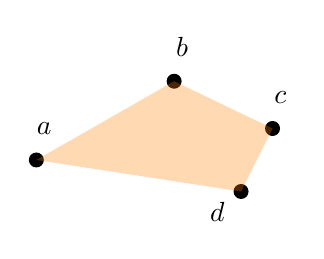
\begin{tikzpicture}
            \node[draw, circle, black, fill=black, inner sep=0pt, minimum size=5pt, label={[xshift=0.1cm, yshift=0.1cm]$a$}] (a) at (0,0) {};
            \node[draw, circle, black, fill=black, inner sep=0pt, minimum size=5pt, label={[xshift=0.1cm, yshift=0.1cm]$b$}] (b) at (1.75,1) {};
            \node[draw, circle, black, fill=black, inner sep=0pt, minimum size=5pt, label={[xshift=0.1cm, yshift=0.1cm]$c$}] (c) at (3,0.4) {};
            \node[draw, circle, black, fill=black, inner sep=0pt, minimum size=5pt, label={[xshift=-0.3cm, yshift=-0.6cm]$d$}] (d) at (2.6,-0.4) {};
            \coordinate (a) at (0,0);
            \coordinate (b) at (1.75,1);
            \coordinate (c) at (3,0.4);
            \coordinate (d) at (2.6,-0.4);
            \fill[orange, opacity=0.3] (a) -- (b) -- (c) -- (d) -- (a) -- cycle;
        \end{tikzpicture}
        \caption{The signature induced by $\sigma$ is $\texttt{-\,-\,-\,-}$.}
    \end{subfigure}
    \begin{subfigure}{0.3\linewidth}
        \centering
        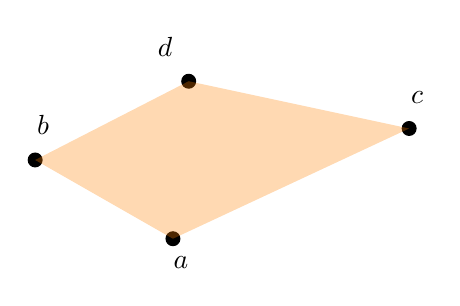
\begin{tikzpicture}
            \node[draw, circle, black, fill=black, inner sep=0pt, minimum size=5pt, label={[xshift=0.1cm, yshift=-0.6cm]$a$}] (a) at (0,0) {};
            \node[draw, circle, black, fill=black, inner sep=0pt, minimum size=5pt, label={[xshift=0.1cm, yshift=0.1cm]$b$}] (b) at (-1.75,1) {};
            \node[draw, circle, black, fill=black, inner sep=0pt, minimum size=5pt, label={[xshift=0.1cm, yshift=0.1cm]$c$}] (c) at (3,1.4) {};
            \node[draw, circle, black, fill=black, inner sep=0pt, minimum size=5pt, label={[xshift=-0.3cm, yshift=0.1cm]$d$}] (d) at (0.2,2) {};
            \coordinate (a) at (0,0);
            \coordinate (b) at (-1.75,1);
            \coordinate (c) at (3,1.4);
            \coordinate (d) at (0.2,2);
            \fill[orange, opacity=0.3] (b) -- (d) -- (c) -- (a) -- (b) -- cycle;
        \end{tikzpicture}
        \caption{The signature induced by $\sigma$ is $\texttt{-\,-\,+\,-}$.}
    \end{subfigure}
    \begin{subfigure}{0.3\linewidth}
        \centering
        
\begin{tikzpicture}
            \node[draw, circle, black, fill=black, inner sep=0pt, minimum size=5pt] (p) at (0,0) {};
        \end{tikzpicture}
    \end{subfigure}
  \caption{Illustration of the notion of $\sigma$-equivalence.}\label{fig:sigma-equiv}
  \end{figure}


Third, the lex-order property breaks symmetry due to \emph{reflection}.
Reflecting a set of points~$S$ over a line (e.g., with the map $(x, y) \mapsto (-x, y)$)
preserves the presence of $k$-holes and convex $k$-gons.
This operation does not quite preserve orientations, but rather flips them
(clockwise orientations become counterclockwise and vice versa).
Our definition of $\sigma$-equivalence includes a \emph{parity} flag for this purpose:
\lstinline|parity := false| corresponds to the case that orientations are the same,
and \lstinline|parity := true| corresponds to the case that all orientations have been flipped.
See the point sets in \Cref{fig:sigma-equiv} for an example.

The lex-order property, then, picks between a set of points and its reflection over \(x=0\).
The vector of consecutive orientations from the middle to the left
is assumed to be at least as big as the vector of consecutive orientations from the middle to the right.
This constraint is not geometrically meaningful,
but is easy to implement in the SAT encoding.

We prove that there always exists a $\sigma$-equivalent point set in canonical position.

%     While the first 3 conditions are now arguably standard in computational results regarding Erd\H{o}s-Szekeres type problems~\cite{scheucherTwoDisjoint5holes2020}, the last condition is a novelty introduced by Heule and Scheucher.
%     Interestingly, in the process of verifying the correctness of this symmetry-breaking assumption, we found a small error in the proof presented in~\cite{scheucherTwoDisjoint5holes2020} for the first $3$ conditions.
% The concrete theorem we prove is the following:
\begin{figure}[t]
\begin{subfigure}{0.31\textwidth}
\centering
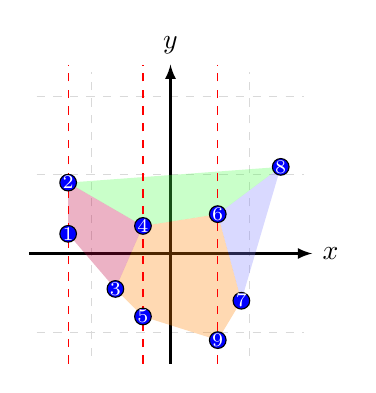
\begin{tikzpicture}
        \draw[help lines, color=gray!30, dashed] (-1.7,-1.3) grid (1.7,2.3);
    \draw[-latex, thick] (-1.8,0)--(1.8,0) node[right]{$x$};
    \draw[-latex, thick] (0,-1.4)--(0,2.4) node[above]{$y$};

    \coordinate (c1) at (-1.3, 0.25);
    \coordinate (c2) at (-1.3, 0.9);
    \coordinate (c3) at (-0.7, -0.45);
    \coordinate (c4) at (-0.35, 0.35);
    \coordinate (c5) at (-0.35, -0.8);
    \coordinate (c6) at (0.6, 0.5);
    \coordinate (c7) at (0.9, -0.6);
    \coordinate (c8) at (1.4, 1.1);
    \coordinate (c9) at (0.6, -1.1);
    
    \fill[orange, opacity=0.3] (c3) -- (c4) -- (c6) -- (c7) -- (c9) -- (c5) -- (c3) -- cycle;
    \fill[purple, opacity=0.3] (c2) -- (c4) -- (c3) -- (c1) -- (c2) -- cycle;
    \fill[blue!50!white, opacity=0.3] (c6) -- (c7) -- (c8) -- (c6) -- cycle;
    \fill[green!70!white, opacity=0.3] (c2) -- (c4) -- (c6) -- (c8) -- (c2) -- cycle;
 
    \draw[-, dashed, red] (-1.3, -1.4) -- (-1.3, 2.4);
    \draw[-, dashed, red] (-0.35, -1.4) -- (-0.35, 2.4);
    \draw[-, dashed, red] (0.6, -1.4) -- (0.6, 2.4);
    \node[draw, circle, fill=blue, text=white, inner sep=0pt, minimum size=5pt] (p1) at (-1.3, 0.25) {\scriptsize $1$};
    \node[draw, circle, fill=blue, text=white, inner sep=0pt, minimum size=5pt] (p2) at (-1.3, 0.9) {\scriptsize $2$};
    \node[draw, circle, fill=blue, text=white, inner sep=0pt, minimum size=5pt] (p3) at (-0.7, -0.45) {\scriptsize $3$};
    \node[draw, circle, fill=blue, text=white, inner sep=0pt, minimum size=5pt] (p4) at (-0.35, 0.35) {\scriptsize $4$};
    \node[draw, circle, fill=blue, text=white, inner sep=0pt, minimum size=5pt] (p5) at (-0.35, -0.8) {\scriptsize $5$};
    \node[draw, circle, fill=blue, text=white, inner sep=0pt, minimum size=5pt] (p6) at (0.6, 0.5) {\scriptsize $6$};
    \node[draw, circle, fill=blue, text=white, inner sep=0pt, minimum size=5pt] (p7) at (0.9, -0.6) {\scriptsize $7$};
    \node[draw, circle, fill=blue, text=white, inner sep=0pt, minimum size=5pt] (p8) at (1.4, 1.1) {\scriptsize $8$};
    \node[draw, circle, fill=blue, text=white, inner sep=0pt, minimum size=5pt] (p9) at (0.6, -1.1) {\scriptsize $9$};
\end{tikzpicture}
\caption{The original list of points.\\\phantom{x}\\\phantom{x}}\label{fig:symmetry-breaking-1}
\end{subfigure}
\hfil
\begin{subfigure}{0.31\textwidth}
    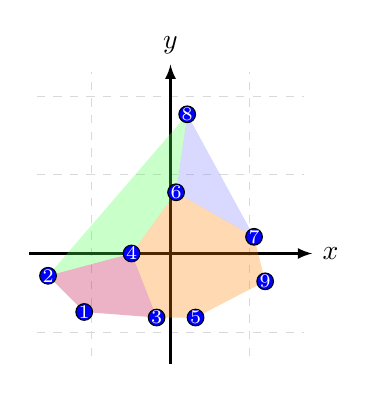
\begin{tikzpicture}
        \draw[help lines, color=gray!30, dashed] (-1.7,-1.3) grid (1.7,2.3);
    \draw[-latex, thick] (-1.8,0)--(1.8,0) node[right]{$x$};
    \draw[-latex, thick] (0,-1.4)--(0,2.4) node[above]{$y$};
    

    \coordinate (c1) at (-1.09601563215555, -0.7424619411597272);
\coordinate (c2) at (-1.5556349648261614, -0.28284245828783905);
\coordinate (c3) at (-0.17677682816699475, -0.8131727694796578);
\coordinate (c4) at (-0.49497474683057663, 8.087761060870946e-08);
\coordinate (c5) at (0.3181979186635819, -0.8131728503572684);
\coordinate (c6) at (0.07071080521204193, 0.7778174477512475);
\coordinate (c7) at (1.0606602064416402, 0.21213186104679588);
\coordinate (c8) at (0.21213232320457065, 1.767766918304512);
\coordinate (c9) at (1.202081470247393, -0.3535535870103234);

\fill[orange, opacity=0.3] (c3) -- (c4) -- (c6) -- (c7) -- (c9) -- (c5) -- (c3) -- cycle;
\fill[purple, opacity=0.3] (c2) -- (c4) -- (c3) -- (c1) -- (c2) -- cycle;
\fill[blue!50!white, opacity=0.3] (c6) -- (c7) -- (c8) -- (c6) -- cycle;
\fill[green!70!white, opacity=0.3] (c2) -- (c4) -- (c6) -- (c8) -- (c2) -- cycle;

        \node[draw, circle, fill=blue, text=white, inner sep=0pt, minimum size=5pt] (p1) at (-1.09601563215555, -0.7424619411597272) {\scriptsize $1$};
        \node[draw, circle, fill=blue, text=white, inner sep=0pt, minimum size=5pt] (p2) at (-1.5556349648261614, -0.28284245828783905) {\scriptsize $2$};
        \node[draw, circle, fill=blue, text=white, inner sep=0pt, minimum size=5pt] (p3) at (-0.17677682816699475, -0.8131727694796578) {\scriptsize $3$};
        \node[draw, circle, fill=blue, text=white, inner sep=0pt, minimum size=5pt] (p4) at (-0.49497474683057663, 8.087761060870946e-08) {\scriptsize $4$};
        \node[draw, circle, fill=blue, text=white, inner sep=0pt, minimum size=5pt] (p5) at (0.3181979186635819, -0.8131728503572684) {\scriptsize $5$};
        \node[draw, circle, fill=blue, text=white, inner sep=0pt, minimum size=5pt] (p6) at (0.07071080521204193, 0.7778174477512475) {\scriptsize $6$};
        \node[draw, circle, fill=blue, text=white, inner sep=0pt, minimum size=5pt] (p7) at (1.0606602064416402, 0.21213186104679588) {\scriptsize $7$};
        \node[draw, circle, fill=blue, text=white, inner sep=0pt, minimum size=5pt] (p8) at (0.21213232320457065, 1.767766918304512) {\scriptsize $8$};
        \node[draw, circle, fill=blue, text=white, inner sep=0pt, minimum size=5pt] (p9) at (1.202081470247393, -0.3535535870103234) {\scriptsize $9$};
    \end{tikzpicture}

\caption{All $x$-coordinates are different after rotating by $45^\circ$. We show such an angle always exists.}\label{fig:symmetry-breaking-2}
\end{subfigure}
\hfil
%
%\vspace{0.5cm}
%
\begin{subfigure}{0.31\textwidth}
    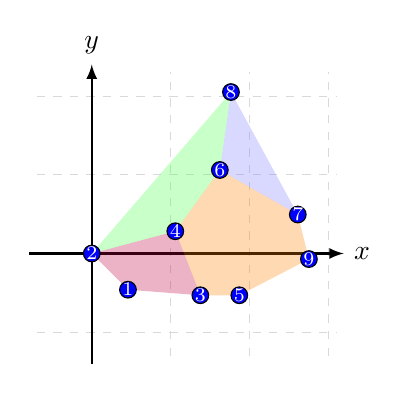
\begin{tikzpicture}
            \draw[help lines, color=gray!30, dashed] (-0.7,-1.3) grid (3.1,2.3);
    \draw[-latex, thick] (-0.8,0)--(3.2,0) node[right]{$x$};
    \draw[-latex, thick] (0,-1.4)--(0,2.4) node[above]{$y$};
    
    \coordinate (c1) at (0.4596193326706113, -0.45961948287188814);
\coordinate (c2) at (0.0, 0.0);
\coordinate (c3) at (1.3788581366591666, -0.5303303111918187);
\coordinate (c4) at (1.0606602179955846, 0.28284253916544966);
\coordinate (c5) at (1.8738328834897433, -0.5303303920694293);
\coordinate (c6) at (1.6263457700382034, 1.0606599060390867);
\coordinate (c7) at (2.6162951712678018, 0.4949743193346349);
\coordinate (c8) at (1.767767288030732, 2.0506093765923508);
\coordinate (c9) at (2.7577164350735544, -0.07071112872248436);

\fill[orange, opacity=0.3] (c3) -- (c4) -- (c6) -- (c7) -- (c9) -- (c5) -- (c3) -- cycle;
\fill[purple, opacity=0.3] (c2) -- (c4) -- (c3) -- (c1) -- (c2) -- cycle;
\fill[blue!50!white, opacity=0.3] (c6) -- (c7) -- (c8) -- (c6) -- cycle;
\fill[green!70!white, opacity=0.3] (c2) -- (c4) -- (c6) -- (c8) -- (c2) -- cycle;
%        \draw[help lines, color=gray!30, dashed] (-1,-0.9) grid (2.9,2.4);
%        \draw[-latex, thick] (-1,0)--(4,0) node[right]{$x$};
%        \draw[-latex, thick] (0,-1)--(0,2.5) node[above]{$y$};
    
        \node[draw, circle, fill=blue, text=white, inner sep=0pt, minimum size=5pt] (p1) at (0.4596193326706113, -0.45961948287188814) {\scriptsize $1$};
        \node[draw, circle, fill=blue, text=white, inner sep=0pt, minimum size=5pt] (p2) at (0.0, 0.0) {\scriptsize $2$};
        \node[draw, circle, fill=blue, text=white, inner sep=0pt, minimum size=5pt] (p3) at (1.3788581366591666, -0.5303303111918187) {\scriptsize $3$};
        \node[draw, circle, fill=blue, text=white, inner sep=0pt, minimum size=5pt] (p4) at (1.0606602179955846, 0.28284253916544966) {\scriptsize $4$};
        \node[draw, circle, fill=blue, text=white, inner sep=0pt, minimum size=5pt] (p5) at (1.8738328834897433, -0.5303303920694293) {\scriptsize $5$};
        \node[draw, circle, fill=blue, text=white, inner sep=0pt, minimum size=5pt] (p6) at (1.6263457700382034, 1.0606599060390867) {\scriptsize $6$};
        \node[draw, circle, fill=blue, text=white, inner sep=0pt, minimum size=5pt] (p7) at (2.6162951712678018, 0.4949743193346349) {\scriptsize $7$};
        \node[draw, circle, fill=blue, text=white, inner sep=0pt, minimum size=5pt] (p8) at (1.767767288030732, 2.0506093765923508) {\scriptsize $8$};
        \node[draw, circle, fill=blue, text=white, inner sep=0pt, minimum size=5pt] (p9) at (2.7577164350735544, -0.07071112872248436) {\scriptsize $9$};
    \end{tikzpicture}

\caption{After translating, the leftmost point is at $(0,0)$.\\\phantom{x}}\label{fig:symmetry-breaking-3}
\end{subfigure}

\begin{subfigure}{0.31\textwidth}
    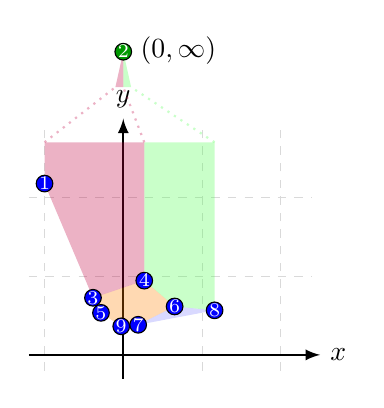
\begin{tikzpicture}
        \draw[help lines, color=gray!30, dashed] (-1.2,-0.2) grid (2.4,2.9);
        \draw[-latex, thick] (-1.2,0)--(2.5,0) node[right]{$x$};
        \draw[-latex, thick] (0,-0.3)--(0,3) node[above]{$y$};
    
        \coordinate (c1) at (-1.00000032679495, 2.1757135283877527);
\coordinate (c2) at (0, 3.85);
\coordinate (c2-1) at (-1.00000032679495, 2.7);
\coordinate (c2-4) at (0.2666664916498519, 2.7);
\coordinate (c2-8) at (1.1599996167350177, 2.7);
\coordinate (t-c2-1) at (-0.1, 3.4);
\coordinate (t-c2-4) at (0, 3.4);
\coordinate (t-c2-8) at (0.1, 3.4);
\coordinate (c3) at (-0.3846155721840648, 0.7252377698715973);
\coordinate (c4) at (0.2666664916498519, 0.9428090005013866);
\coordinate (c5) at (-0.2830190444100679, 0.5336655199142649);
\coordinate (c6) at (0.6521736801480853, 0.6148753963780468);
\coordinate (c7) at (0.1891890199433349, 0.3822198699068886);
\coordinate (c8) at (1.1599996167350177, 0.5656853177286622);
\coordinate (c9) at (-0.025641189145902285, 0.3626188636662086);

\fill[orange, opacity=0.3] (c3) -- (c4) -- (c6) -- (c7) -- (c9) -- (c5) -- (c3) -- cycle;
\fill[blue!50!white, opacity=0.3] (c6) -- (c7) -- (c8) -- (c6) -- cycle;
\fill[purple, opacity=0.3] (c2-4) -- (c4) -- (c3) -- (c1) -- (c2-1) -- cycle;
\fill[purple, opacity=0.3] (t-c2-1) -- (c2) -- (t-c2-4) -- (t-c2-1) -- cycle;
\fill[green!70!white, opacity=0.3] (t-c2-4) -- (c2) -- (t-c2-8) -- (t-c2-4) -- cycle;
\fill[green!70!white, opacity=0.3] (c2-4) -- (c4) -- (c6) -- (c8) -- (c2-8) -- cycle;

\draw[thick, dotted,purple, opacity=0.3] (c2-1) -- (t-c2-1);
\draw[thick, dotted, purple, opacity=0.3] (c2-4) -- (t-c2-4);
\draw[thick, dotted, green!70!white, opacity=0.3] (c2-8) -- (t-c2-8);


        \node[draw, circle, fill=blue, text=white, inner sep=0pt, minimum size=5pt] (p1) at (-1.00000032679495, 2.1757135283877527) {\scriptsize $1$};
        \node[draw, circle, fill=green!60!black, text=white, inner sep=0pt, minimum size=5pt, label={[xshift=0.7cm, yshift=-0.4cm]$(0, \infty)$}] (p2) at (0, 3.85) {\scriptsize $2$};
        \node[draw, circle, fill=blue, text=white, inner sep=0pt, minimum size=5pt] (p3) at (-0.3846155721840648, 0.7252377698715973) {\scriptsize $3$};
        \node[draw, circle, fill=blue, text=white, inner sep=0pt, minimum size=5pt] (p4) at (0.2666664916498519, 0.9428090005013866) {\scriptsize $4$};
        \node[draw, circle, fill=blue, text=white, inner sep=0pt, minimum size=5pt] (p5) at (-0.2830190444100679, 0.5336655199142649) {\scriptsize $5$};
        \node[draw, circle, fill=blue, text=white, inner sep=0pt, minimum size=5pt] (p6) at (0.6521736801480853, 0.6148753963780468) {\scriptsize $6$};
        \node[draw, circle, fill=blue, text=white, inner sep=0pt, minimum size=5pt] (p7) at (0.1891890199433349, 0.3822198699068886) {\scriptsize $7$};
        \node[draw, circle, fill=blue, text=white, inner sep=0pt, minimum size=5pt] (p8) at (1.1599996167350177, 0.5656853177286622) {\scriptsize $8$};
        \node[draw, circle, fill=blue, text=white, inner sep=0pt, minimum size=5pt] (p9) at (-0.025641189145902285, 0.3626188636662086) {\scriptsize $9$};
       
    \end{tikzpicture}

\caption{Result after applying the map $(x, y) \mapsto (y/x, 1/x)$.}\label{fig:symmetry-breaking-4}
\end{subfigure}
\hfil
%
%\vspace{0.5cm}
%
\begin{subfigure}{0.31\textwidth}
    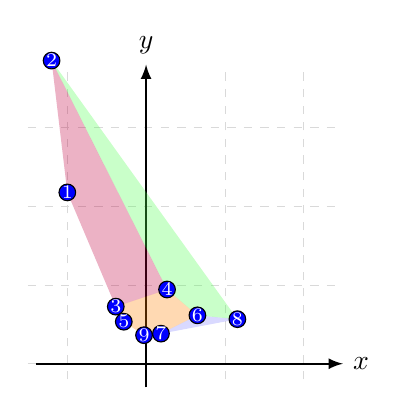
\begin{tikzpicture}
        \draw[help lines, color=gray!30, dashed] (-1.5,-0.2) grid (2.4,3.7);
        \draw[-latex, thick] (-1.4,0)--(2.5,0) node[right]{$x$};
        \draw[-latex, thick] (0,-0.3)--(0,3.8) node[above]{$y$};
    
        \coordinate (c1) at (-1.00000032679495, 2.1757135283877527);
        \coordinate (c2) at (-1.2, 3.85);
        \coordinate (c3) at (-0.3846155721840648, 0.7252377698715973);
        \coordinate (c4) at (0.2666664916498519, 0.9428090005013866);
        \coordinate (c5) at (-0.2830190444100679, 0.5336655199142649);
        \coordinate (c6) at (0.6521736801480853, 0.6148753963780468);
        \coordinate (c7) at (0.1891890199433349, 0.3822198699068886);
        \coordinate (c8) at (1.1599996167350177, 0.5656853177286622);
        \coordinate (c9) at (-0.025641189145902285, 0.3626188636662086);
   
        \fill[orange, opacity=0.3] (c3) -- (c4) -- (c6) -- (c7) -- (c9) -- (c5) -- (c3) -- cycle;
        \fill[blue!50!white, opacity=0.3] (c6) -- (c7) -- (c8) -- (c6) -- cycle;
        \fill[purple, opacity=0.3] (c2) -- (c4) -- (c3) -- (c1) -- (c2) -- cycle;
        \fill[green!70!white, opacity=0.3] (c2) -- (c4) -- (c6) -- (c8) -- (c2) -- cycle;

        \node[draw, circle, fill=blue, text=white, inner sep=0pt, minimum size=5pt] (p1) at (-1.00000032679495, 2.1757135283877527) {\scriptsize $1$};
        \node[draw, circle, fill=blue, text=white, inner sep=0pt, minimum size=5pt] (p2) at (-1.2, 3.85) {\scriptsize $2$};
        \node[draw, circle, fill=blue, text=white, inner sep=0pt, minimum size=5pt] (p3) at (-0.3846155721840648, 0.7252377698715973) {\scriptsize $3$};
        \node[draw, circle, fill=blue, text=white, inner sep=0pt, minimum size=5pt] (p4) at (0.2666664916498519, 0.9428090005013866) {\scriptsize $4$};
        \node[draw, circle, fill=blue, text=white, inner sep=0pt, minimum size=5pt] (p5) at (-0.2830190444100679, 0.5336655199142649) {\scriptsize $5$};
        \node[draw, circle, fill=blue, text=white, inner sep=0pt, minimum size=5pt] (p6) at (0.6521736801480853, 0.6148753963780468) {\scriptsize $6$};
        \node[draw, circle, fill=blue, text=white, inner sep=0pt, minimum size=5pt] (p7) at (0.1891890199433349, 0.3822198699068886) {\scriptsize $7$};
        \node[draw, circle, fill=blue, text=white, inner sep=0pt, minimum size=5pt] (p8) at (1.1599996167350177, 0.5656853177286622) {\scriptsize $8$};
        \node[draw, circle, fill=blue, text=white, inner sep=0pt, minimum size=5pt] (p9) at (-0.025641189145902285, 0.3626188636662086) {\scriptsize $9$};
       
       

    \end{tikzpicture}

\caption{Point $2$ is brought back into the real plane.}\label{fig:symmetry-breaking-5}
\end{subfigure}
\hfil
\begin{subfigure}{0.31\textwidth}
    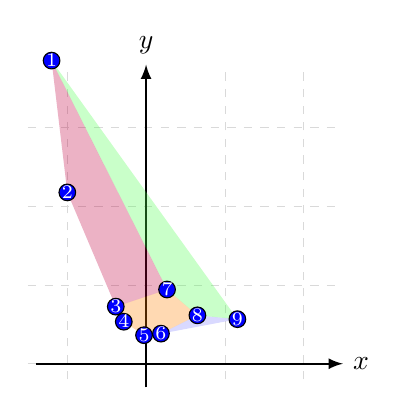
\begin{tikzpicture}
        \draw[help lines, color=gray!30, dashed] (-1.5,-0.2) grid (2.4,3.7);
        \draw[-latex, thick] (-1.4,0)--(2.5,0) node[right]{$x$};
        \draw[-latex, thick] (0,-0.3)--(0,3.8) node[above]{$y$};
    
        \coordinate (c1) at (-1.00000032679495, 2.1757135283877527);
        \coordinate (c2) at (-1.2, 3.85);
        \coordinate (c3) at (-0.3846155721840648, 0.7252377698715973);
        \coordinate (c4) at (0.2666664916498519, 0.9428090005013866);
        \coordinate (c5) at (-0.2830190444100679, 0.5336655199142649);
        \coordinate (c6) at (0.6521736801480853, 0.6148753963780468);
        \coordinate (c7) at (0.1891890199433349, 0.3822198699068886);
        \coordinate (c8) at (1.1599996167350177, 0.5656853177286622);
        \coordinate (c9) at (-0.025641189145902285, 0.3626188636662086);
        
        \fill[orange, opacity=0.3] (c3) -- (c4) -- (c6) -- (c7) -- (c9) -- (c5) -- (c3) -- cycle;
        \fill[blue!50!white, opacity=0.3] (c6) -- (c7) -- (c8) -- (c6) -- cycle;
        \fill[purple, opacity=0.3] (c2) -- (c4) -- (c3) -- (c1) -- (c2) -- cycle;
    \fill[green!70!white, opacity=0.3] (c2) -- (c4) -- (c6) -- (c8) -- (c2) -- cycle;

        \node[draw, circle, fill=blue, text=white, inner sep=0pt, minimum size=5pt] (p1) at (-1.2, 3.85) {\scriptsize $1$};
        \node[draw, circle, fill=blue, text=white, inner sep=0pt, minimum size=5pt] (p2) at (-1.00000032679495, 2.1757135283877527) {\scriptsize $2$};
        \node[draw, circle, fill=blue, text=white, inner sep=0pt, minimum size=5pt] (p3) at (-0.3846155721840648, 0.7252377698715973) {\scriptsize $3$};
        \node[draw, circle, fill=blue, text=white, inner sep=0pt, minimum size=5pt] (p4) at (-0.2830190444100679, 0.5336655199142649) {\scriptsize $4$};
        \node[draw, circle, fill=blue, text=white, inner sep=0pt, minimum size=5pt] (p5) at (-0.025641189145902285, 0.3626188636662086) {\scriptsize $5$};
        \node[draw, circle, fill=blue, text=white, inner sep=0pt, minimum size=5pt] (p6) at (0.1891890199433349, 0.3822198699068886) {\scriptsize $6$};
        \node[draw, circle, fill=blue, text=white, inner sep=0pt, minimum size=5pt] (p7) at (0.2666664916498519, 0.9428090005013866) {\scriptsize $7$};
        \node[draw, circle, fill=blue, text=white, inner sep=0pt, minimum size=5pt] (p8) at (0.6521736801480853, 0.6148753963780468) {\scriptsize $8$};
        \node[draw, circle, fill=blue, text=white, inner sep=0pt, minimum size=5pt] (p9) at (1.1599996167350177, 0.5656853177286622) {\scriptsize $9$};
       
    \end{tikzpicture}

\caption{Points are relabeled from left to right.}\label{fig:symmetry-breaking-6}
\end{subfigure}



\caption{Illustration of the proof of the symmetry breaking theorem. Note that the highlighted holes are preserved as $\sigma$-equivalence is preserved. For simplicity we have ommited the illustration of the \emph{Lex-order} property. }\label{fig:symmetry-breaking}
\end{figure}
\begin{lstlisting}
theorem symmetry_breaking : ListInGenPos l →
  ∃ w : CanonicalPoints, Nonempty (l.toFinset ≃σ w.points.toFinset)
\end{lstlisting}


\begin{proof}[Proof Sketch]
The proof proceeds in 6 steps, illustrated in~\Cref{fig:symmetry-breaking}.
In each of the steps, we will construct a new list of points that is $\sigma$-equivalent to the previous one,
and the last one will be in canonical position.
\footnote{Even though we defined $\sigma$-equivalence for sets of points,
our formalization goes back and forth between sets and lists.
Given that symmetry breaking distinguishes between the order of the points
e.g., $x$-order, this proof proceeds over lists.
All permutations of a list are immediately $\sigma$-equivalent.}
The main justification for each step is that,
given that the function $\sigma$ is defined as a sign of the determinant,
applying transformations that preserve (or, when \lstinline|parity := true|, uniformly reverse)
the sign of the determinant will preserve (or uniformly reverse) the values of $\sigma$.

For example, given the identity $\det(AB) = \det(A)\det(B)$,
if we apply a transformation to the points that corresponds to multiplying by a matrix $B$ such that $\det(B) > 0$,
then $\sign(\det(A)) = \sign(\det(AB))$, and thus orientations will be preserved.
\textbf{Step 1}: we transform the list of points so that no two points share the same $x$-coordinate.
This can be done by applying a rotation to the list of points, which corresponds to multiplying by a rotation matrix.
Rotations always have determinant $1$.
\textbf{Step 2}: we translate all points by a constant vector $t$, by multiplying by a translation matrix,
so that the left most point gets position $(0, 0)$, and naturally every other point will have a positive $x$-coordinate.

Let $L_2$ be the list of points after Step 2, excluding $(0,0)$ which we will denote by $p_1$.
\textbf{Step 3}: we apply the projective transformation $f: (x, y) \mapsto (y/x, 1/x)$ to every point in $L_2$,
showing that this preserves orientations within $L_2$.
To see that this mapping is a $\sigma$-equivalence consider that
\[
\begin{multlined}
 \sign \det \begin{pmatrix} p_x & q_x & r_x \\ p_y & q_y & r_y \\ 1 & 1 & 1 \end{pmatrix} =  \sign \det \left( \begin{pmatrix} 0 & 0 & 1 \\ 1 & 0 & 0\\ 0 & 1 & 0 \end{pmatrix}  \begin{pmatrix} \nicefrac{p_y}{p_x} & \nicefrac{q_y}{q_x} & \nicefrac{r_y}{r_x} \\ \nicefrac{1}{p_x} & \nicefrac{1}{q_x} & \nicefrac{1}{r_x} \\ 1 & 1 & 1 \end{pmatrix}  \begin{pmatrix} p_x & 0 & 0 \\ 0 & q_x & 0\\ 0 & 0 & r_x \end{pmatrix} \right)\\
                        = \sign \left(1 \cdot \det  \begin{pmatrix} \nicefrac{p_y}{p_x} & \nicefrac{q_y}{q_x} & \nicefrac{r_y}{r_x} \\ \nicefrac{1}{p_x} & \nicefrac{1}{q_x} & \nicefrac{1}{r_x} \\ 1 & 1 & 1 \end{pmatrix} \cdot  p_x q_x r_x  \right) = \sign \det \begin{pmatrix} p_y/p_x & q_y/q_x & r_y/r_x \\ 1/p_x & 1/q_x & 1/r_x \\ 1 & 1 & 1 \end{pmatrix}.
                        %  \tag{As $p_x q_x r_x > 0$ by step 2}
\end{multlined}
\]
To preserve orientations with respect to the leftmost point $(0, 0)$, we set $f( (0, 0)) = (0, \infty)$,
a special point that is treated separately as follows.
As the function $\sigma$ takes points in $\mathbb{R}^2$ as arguments,
we need to define an extension
\(
  \sigma_{(0, \infty)}(q, r) = \begin{cases}
    1 & \text{if } q_x < r_x \\
    -1 & \text{otherwise}.  
  \end{cases},
\)
We then show that $\sigma((0, 0), q, r) = \sigma_{(0, \infty)}(f(q), f(r))$ for all points $q, r \in L_2$. 

\textbf{Step 4}: we sort the list $L_2$ by $x$-coordinate in increasing order,
thus obtaining a list $L_3$.
This can be done while preserving $\sigma$-equivalence because sorting corresponds to a permutation,
and all permutations of a list are $\sigma$-equivalent by definition.
\textbf{Step 5}: we check whether the \textsf{Lex order} condition above is satisfied in $L_3$,
and if it is not, we reflect the pointset,
which preserves $\sigma$-equivalence with \lstinline|parity := true|.
Note that in such a case we need to relabel the points from left to right again.

\textbf{Step 6}: we bring point $(0, \infty)$ back into the range
by first finding a constant $c$ such that all points in $L_3$ are to the right of the line $y=c$,
and then finding a large enough value $M$ such that $(c, M)$ has the same orientation
with respect to the other points as $(0, \infty)$ did,
meaning that 
\(\sigma((c, M), q, r) = \sigma_{(0, \infty)}(q, r)\) for every $q, r \in L_3$.

Finally, we note that the list of points obtained in step 6
satisfies the \text{CCW-order} property by the following reasoning:
if $1 < i < j \leq n$ are indices, then 
\begin{align*}
  \sigma(p_1, p_i, p_j) = 1 &\iff \sigma((c, M), p_i, p_j) = 1\\
                            &\iff \sigma_{(0, \infty)}(p_i, p_j) = 1\tag{By step 6}\\
                            &\iff (p_i)_x < (p_j)_x \tag{By definition of $\sigma_{(0, \infty)}$}\\
                            &\iff \textsf{true} \tag{By step 4, since points are sorted and $i < j$}.
\end{align*}
This concludes the proof.
\end{proof}

We had quite some difficulty formalizing the symmetry-breaking argument.
We spent many hours around a whiteboard,
simplifying the argument to minimize the amount of theory we would need to develop.
The projective transformation in Step 3 was particularly difficult to wrangle.
This step, and those after it, requires careful bookkeeping around the distinguished point $p_1$.

Once these details were worked out,
the proof was relatively straightforward, albeit long and tedious.
Each step of the proof justifies not only that a new property is achieved,
but also that all properties from previous steps are preserved.
As a result, the proof burden was substantial.


\section{Encoding and Correctness}\label{sec:encoding}
Having established the reduction to orientations,
and the symmetry-breaking assumption of canonicity,
we now turn to the construction of a CNF formula $\phi_n$
whose unsatisfiability would imply
that every set of $n$ points
contains a $6$-hole.\footnote{
  Satisfiability of $\phi_n$ would \emph{not} necessarily imply
  the existence of a point set without a $6$-hole, due to the \emph{realizability problem} (see e.g.,~\cite{subercaseaux2023minimizing}).
  % First, the mapping from sets of points to assignments of triple orientations is not surjective.
  % Second, even if it were, $\phi_n$ is tailored to looking for an unsatisfiability proof,
  % using implication rather than bi-implication in some of the variable-defining clauses.
}
The formula is detailed in~\Cref{fig:full-encoding}.

\begin{figure}
  \label{fig:full-encoding}
% \begin{framed}
  \begin{spreadlines}{16pt}
\begin{gather}
\hfsetfillcolor{green!10}
\hfsetbordercolor{green!60!black}
\tikzmarkin{b}(12.0,-0.9)(-0.5,0.5)
  \cvar_{i; a,b, c} \rightarrow \left(\left(\orvar_{a,b,c} \leftrightarrow \orvar_{a, i, c}  \right) \land \left(\orvar_{a,b,c} \leftrightarrow \ov{\orvar_{a, i, b}}  \right)\right) \text{ for all } 2 \leq a < i < b < c \leq n\label{eq:insideClauses1}\\
  \cvar_{i; a,b, c} \rightarrow \left(\left(\orvar_{a,b,c} \leftrightarrow \orvar_{a, i, c}  \right) \land \left(\orvar_{a,b,c} \leftrightarrow \ov{\orvar_{b, i, c}}  \right)\right) \text{ for all } 2 \leq a < b < i < c \leq n\label{eq:insideClauses2}\\
  \tikzmarkend{b}\Big(\bigwedge_{\substack{a < i < c\\ i \neq b}} \ov{\cvar_{i; a,b,c}}\Big) \rightarrow \hvar_{a, b, c} \quad \text{ for all } 2 \leq a < b < c \leq n\label{eq:holeDefClauses1}\\
%
\tikzmarkin{a}(12.0,-0.3)(-0.5,0.5)
  \orvar_{a, b, c} \land \orvar_{a, c, d} \rightarrow \orvar_{a, b, d} \quad \text{ for all } 2 \leq a < b < c < d \leq n\label{eq:signotopeClauses11}\\
  \tikzmarkend{a}\ov{\orvar_{a, b, c}} \land \ov{\orvar_{a, c, d}} \rightarrow \ov{\orvar_{a, b, d}} \quad \text{ for all } 2 \leq a < b < c < d \leq n \label{eq:signotopeClauses12}\\
%
\hfsetfillcolor{blue!10}
\hfsetbordercolor{blue!60!black}
\tikzmarkin{c}(12.0,-0.4)(-0.5,0.6)
  % \orvar_{1, b, c} \quad \text{ for all } 2 \leq b < c \leq n \label{eq:revLexClauses}\\
  \tikzmarkend{c}\left(\orvar_{\lceil \frac{n}{2} \rceil -1, \lceil \frac{n}{2} \rceil,\lceil \frac{n}{2} \rceil+1}, \ldots, \orvar_{2,3,4} \right) \succeq_{\text{lex}} \left(\orvar_{\lfloor \frac{n}{2}\rfloor +1,  \lfloor \frac{n}{2}\rfloor +2, \lfloor \frac{n}{2}\rfloor +3}, \ldots, \orvar_{n-2, n-1, n} \right)\label{eq:revLexClauses}\\
%
\hfsetfillcolor{orange!10}
\hfsetbordercolor{orange!60!black}
\tikzmarkin{d}(12.0,-0.3)(-0.5,0.5)
  \ov{\orvar_{a,b,c}} \land \ov{\orvar_{b,c,d}} \rightarrow \uvar_{a, c, d} \quad \text{ for all } 2 \leq a < b < c < d \leq n\label{eq:capDef}\\
  \orvar_{a, b, c} \land \orvar_{b, c, d} \rightarrow \vvar_{a, c, d} \quad \text{ for all } 2 \leq a < b < c < d \leq n \label{eq:cupDef}\\
  \uvar_{a,b,c} \land \ov{\orvar_{b,c,d}} \land \hvar_{a,b,d} \rightarrow \ufvar_{a, c, d} \quad \text{ for all } 2 \leq a < b < c < d \leq n,\; a+1<b\label{eq:capFDef}\\
  \uvar_{a, c, d} \rightarrow \ov{\orvar_{a,c,d}} \quad \text{ for all } 2 \leq a < c < d \leq n,\ a+1<c\label{eq:capDef2}\\
  \tikzmarkend{d}\vvar_{a, c, d} \rightarrow \orvar_{a,c,d} \quad \text{ for all } 2 \leq a < c < d \leq n,\; a+1<c\label{eq:cupDef2}\\
%
\hfsetfillcolor{red!10}
\hfsetbordercolor{red!60!black}
\tikzmarkin{e}(12.0,-0.5)(-0.5,0.5)
  \neg(\ufvar_{a,d,e} \land \orvar_{a, p, e}) \quad \text { for all } 2 \leq a < d < e \leq n, \; a < p < e, \; a+2 < d\label{eq:no6Hole1Below}\\
  \neg(\ufvar_{a,d,e} \land \ov{\orvar_{d, e, f}}) \quad \text { for all } 2 \leq a < d < e < f\leq n, \; a+2 < d\label{eq:no6Hole4Above}\\
  \neg(\uvar_{a,c,d} \land \vvar_{a, c', d} \land \hvar_{a,c,c'}) \quad \text{ for all } 2 \leq a < c < c' < d \leq n, \; a+1 < c\label{eq:no6Hole2Below1}\\
  \neg(\uvar_{a,c,d} \land \vvar_{a, c', d} \land \hvar_{a,c',c}) \quad \text{ for all } 2 \leq a < c' < c < d \leq n, \; a+1 < c'\label{eq:no6Hole2Below2}\\
  \tikzmarkend{e}\neg(\vvar_{a,c,d} \land \orvar_{c, d, e} \land \hvar_{a,c,e}) \quad \text{ for all } 2 \leq a < c < d < e \leq n, \; a+1 < c\label{eq:no6Hole3Below}
  \end{gather}
\end{spreadlines}
% \end{framed}
\caption{Encoding based on that of Heule and Scheucher for the Empty Hexagon Number~\cite{emptyHexagonNumber}. Each line determines a set of clauses. Unsatisfiability of the formula below for $n=30$ implies $h(6) \leq 30$, as detailed throughout the paper.}
\end{figure}


\subparagraph*{Variables.}
Let $S = (p_1, \ldots, p_n)$ be the list of points in canonical position.
We explain the variables of $\phi_n$
by specifying their values in the propositional assignment $\tau_S$
that is our intended model of $\phi_n$
corresponding to $S$. We then have:
\begin{itemize}
  \item
    For every $2 \leq a < b < c \leq n$, $\orvar_{a,b,c}$ is true
    iff $\sigma(p_a,p_b,p_c) = +1$.\footnote{
    Since the point set is in general position,
    we have $\neg \orvar_{a,b,c} \iff \sigma(p_a, p_b, p_c) = -1$.}

    The first optimization observes that orientations are antisymmetric:
    if $(p,q,r)$ is counterclockwise then $(q,p,r)$ is clockwise, etc.
    Thus one only needs $\orvar_{a,b,c}$ for ordered triples $(a,b,c)$,
    reducing the number of orientation variables by a factor of $3! = 6$
    relative to using all triples. The second optimization uses the \textbf{CCW-order} property of canonical positions:
    since all $\orvar_{1,a,b}$ are true, we may as well omit them from the encoding.

  \item
    Next, for every $a < b < c$ with $a < i < b$ or $b < i < c$,
    the variable $\cvar_{i;a,b,c}$ is true
    iff \lstinline|σPtInTriangle S[i] S[a] S[b] S[c]| holds.
    By \lstinline|σPtInTriangle_iff|, this is true exactly
    iff $p_i$ is inside the triangle $p_ap_bp_c$.
    The reason for assuming $(a,b,c)$ to be ordered is again symmetry:
    $p_ap_bp_c$ is the same triangle as $p_ap_cp_b$, etc.
    Furthermore thanks to the \textbf{$x$-order} property of canonical positions,
    if $p_i$ is in the triangle
    then $x(p_a) < x(p_i) < x(p_c)$.
    This implies that $a < i < c$,
    leaving one case distinction permuting $(i,b)$.

  \item
    For every $a < b < c$,
    $\hvar_{a,b,c}$ is true
    iff \lstinline|σIsEmptyTriangleFor S[a] S[b] S[c] S| holds.
    %  Analogously to the previous items,
    By a geometro-combinatorial connection analogous to ones above,
    this is true iff $p_ap_bp_c$ is a $3$-hole.

  \item
    Finally, one defines \emph{$4$-cap}, \emph{$5$-cap}, and \emph{$4$-cup} variables.
    For $a+1 < c < d$, $\uvar_{a,c,d}$ is true
    iff there is $b$ with $a < b < c$ with $\sigma(p_a,p_b,p_c) = \sigma(p_b,p_c,p_d) = -1$.
    $\vvar_{a,c,d}$ is analogous, except in that the two orientations are required to be counterclockwise.
    These are the $4$-caps and $4$-cups, respectively.
    The $5$-cap variables $\ufvar_{a,d,e}$
    are defined for $a+2 < d < e$.
    We set $\ufvar_{a,d,e}$ to true
    iff there exists $c$ with $a+1<c<d$
    such that $\uvar_{a,c,d}$, $\orvar_{c,d,e}$, and $\hvar_{a,c,e}$ are all true.
    Intuitively, $4$-caps and $4$-cups are clockwise and counterclockwise arcs of length $4$,
    respectively,
    whereas $5$-caps are clockwise arcs of length $5$ containing a $3$-hole.
    All three are depicted in~\Cref{fig:cup-cap-vars}. The usage of these variables is crucial to an efficient encoding:
    we will show below that a hexagon can be covered by only $4$ triangles,
    so one need not consider all ${6\choose 3}$ triangles contained within it.
\end{itemize}

\begin{figure}
\centering
\begin{subfigure}{0.3\textwidth}
    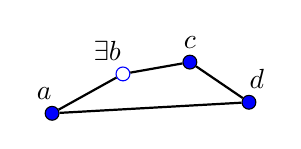
\begin{tikzpicture}
        \node[draw, circle, black, fill=blue, inner sep=0pt, minimum size=5pt,label={[xshift=-0.1cm, yshift=-0.05cm]$a$}] (a) at (0,0) {};
        \node[draw, circle, blue,  inner sep=0pt, minimum size=5pt, label={[xshift=-0.2cm, yshift=-0.05cm]$\exists b$}] (b) at (0.9*1,1*0.5) {};
        \node[draw, circle, black, fill=blue, inner sep=0pt, minimum size=5pt, label={[xshift=-0.0cm, yshift=-0.05cm]$c$}] (c) at (1.75*1, 1.3*0.5) {};
        \node[draw, circle, black, fill=blue, inner sep=0pt, minimum size=5pt, label={[xshift=0.1cm, yshift=-0.05cm]$d$}] (d) at (2.5*1,0.2*0.7) {};
    \draw[thick] (a) -- (b) -- (c) -- (d) -- (a);
    \end{tikzpicture}
    \caption{$\uvar_{a,c,d}$}\label{fig:cap}
\end{subfigure}
\begin{subfigure}{0.3\textwidth}
    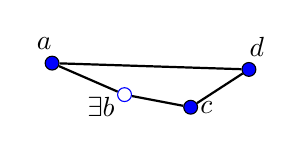
\begin{tikzpicture}
        \node[draw, circle, black, fill=blue, inner sep=0pt, minimum size=5pt,label={[xshift=-0.1cm, yshift=-0.05cm]$a$}] (a) at (0,0) {};
        \node[draw, circle, blue,  inner sep=0pt, minimum size=5pt, label={[xshift=-0.3cm, yshift=-0.5cm]$\exists b$}] (b) at (0.92*1,-0.5*0.8) {};
        \node[draw, circle, black, fill=blue, inner sep=0pt, minimum size=5pt, label={[xshift=0.2cm, yshift=-0.3cm]$c$}] (c) at (1.6*1.1, -0.7*0.8) {};
        \node[draw, circle, black, fill=blue, inner sep=0pt, minimum size=5pt, label={[xshift=0.1cm, yshift=-0.05cm]$d$}] (d) at (2.5*1,-0.2*0.4) {};
    \draw[thick] (a) -- (b) -- (c) -- (d) -- (a);
    \end{tikzpicture}
    \caption{$\vvar_{a,c,d}$}\label{fig:cup}
\end{subfigure}
\begin{subfigure}{0.35\textwidth}
    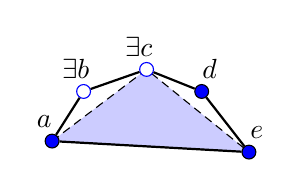
\begin{tikzpicture}
  
    \coordinate (a) at (0,0);
    \coordinate (c) at (1.2*1, 1.3*0.7);
    \coordinate (e) at (2.5*1,-0.2*0.7);
    \fill[blue, opacity=0.2] (a) -- (c) -- (e) -- cycle;
    \draw[densely dashed] (a) -- (c) -- (e) -- (a);

    \node[draw, circle, black, fill=blue, inner sep=0pt, minimum size=5pt,label={[xshift=-0.1cm, yshift=-0.05cm]$a$}] (a) at (0,0) {};
    \node[draw, circle, blue,  fill=white, inner sep=0pt, minimum size=5pt, label={[xshift=-0.1cm, yshift=-0.05cm]$\exists b$}] (b) at (0.4*1,0.9*0.7) {};
    \node[draw, circle, blue, fill=white, inner sep=0pt, minimum size=5pt, label={[xshift=-0.1cm, yshift=-0.05cm]$\exists c$}] (c) at (1.2*1, 1.3*0.7) {};
    \node[draw, circle, black, fill=blue, inner sep=0pt, minimum size=5pt, label={[xshift=0.1cm, yshift=-0.05cm]$d$}] (d) at (1.9*1,0.9*0.7) {};
    \node[draw, circle, black, fill=blue, inner sep=0pt, minimum size=5pt, label={[xshift=0.1cm, yshift=-0.05cm]$e$}] (e) at (2.5*1,-0.2*0.7) {};

    \draw[thick] (a) -- (b) -- (c) -- (d) -- (e) -- (a);
    \end{tikzpicture}
    \caption{$\ufvar_{a,d,e}$}\label{fig:5cap}
\end{subfigure}

\caption{Illustration of the $4$-caps (\ref{fig:cap}), $4$-cups (\ref{fig:cup}), and $5$-caps (\ref{fig:5cap}) variables.  The highlighted region denotes an empty triangle.}\label{fig:cup-cap-vars}
\end{figure}

\begin{figure}
    \centering
    \begin{subfigure}{0.3\textwidth}
        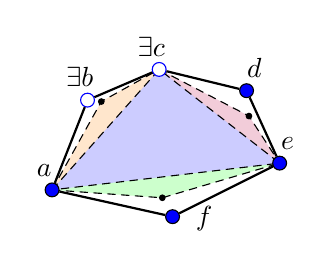
\begin{tikzpicture}
        
    
    
        \coordinate (a) at (0,0);
        \coordinate (c) at (0.8*1.7, 0.9*1.7);
        \coordinate (e) at (1.7*1.7,0.2*1.7);

        \coordinate (p1) at (0.25*2.5, 0.66*1.7);
        \coordinate (p2) at (2.5,0.67*1.4);
        \coordinate (p3) at (1.4,-0.1);

        \fill[blue, opacity=0.2] (a) -- (c) -- (e) -- cycle;
        \fill[orange, opacity=0.2] (a) -- (p1) -- (c) -- cycle;
        \fill[purple, opacity=0.2] (c) -- (p2) -- (e) -- cycle;
        \fill[green, opacity=0.2] (a) -- (p3) -- (e) -- cycle;
        \draw[densely dashed] (a) -- (c) -- (e) -- (a);

        \draw[densely dashed] (a) -- (p1) -- (c);
        \draw[densely dashed] (a) -- (p3) -- (e);
        \draw[densely dashed] (c) -- (p2) -- (e);

        \node[draw, circle, black, fill=blue, inner sep=0pt, minimum size=5pt,label={[xshift=-0.1cm, yshift=-0.05cm]$a$}] (a) at (0,0) {};
        \node[draw, circle, blue, fill=white, inner sep=0pt, minimum size=5pt, label={[xshift=-0.1cm, yshift=-0.05cm]$\exists b$}] (b) at (0.3*1.5,0.6*1.9) {};
        \node[draw, circle, blue, fill=white, inner sep=0pt, minimum size=5pt, label={[xshift=-0.1cm, yshift=-0.05cm]$\exists c$}] (c) at (0.8*1.7, 0.9*1.7) {};
        \node[draw, circle, black, fill=blue, inner sep=0pt, minimum size=5pt, label={[xshift=0.1cm, yshift=-0.05cm]$d$}] (d) at (1.3*1.9,0.7*1.8) {};
        \node[draw, circle, black, fill=blue, inner sep=0pt, minimum size=5pt, label={[xshift=0.1cm, yshift=-0.05cm]$e$}] (e) at (1.7*1.7,0.2*1.7) {};
        \node[draw, circle, black, fill=blue, inner sep=0pt, minimum size=5pt, label={[xshift=0.4cm, yshift=-0.4cm]$f$}] (f) at (0.9*1.7,-0.2*1.7) {};
        \draw[thick] (a) -- (b) -- (c) -- (d) -- (e) -- (f) -- (a);
    
        \node[draw, circle, black, fill=black, inner sep=0pt, minimum size=2pt] (p1) at (0.25*2.5,0.66*1.7) {};
        \node[draw, circle, black, fill=black, inner sep=0pt, minimum size=2pt] (p2) at (2.5,0.67*1.4) {};
        \node[draw, circle, black, fill=black, inner sep=0pt, minimum size=2pt] (p3) at (1.4,-0.1) {};
        \end{tikzpicture}
        \caption{$(\ufvar_{a,d,e} \land \orvar_{a,f,e})$}\label{fig:clause-13-forbid}
    \end{subfigure}
    \begin{subfigure}{0.3\textwidth}
        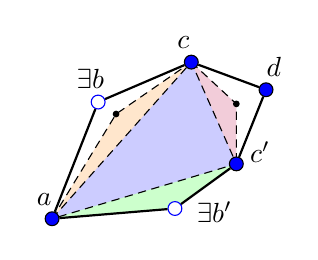
\begin{tikzpicture}
      
       
        \newcommand{\scalefact}{1.3}
        \coordinate (a) at (0*\scalefact,0*\scalefact);
        \coordinate (c) at (0.8*1.7*\scalefact, 0.9*1.7*\scalefact);
        \coordinate (e) at (1.7*1.7*\scalefact,0.2*1.7*\scalefact);

       \coordinate (p1) at (0.25*2.5*\scalefact, 0.66*1.55*\scalefact);
        \coordinate (p2) at (1.8*\scalefact,0.66*1.7*\scalefact);
       \coordinate (bp) at (1.2*\scalefact,0.1*\scalefact);
         \coordinate (cp) at (1.8*\scalefact,0.67*0.8*\scalefact);

        

        \fill[blue, opacity=0.2] (a) -- (c) -- (cp) -- cycle;
        \fill[orange, opacity=0.2] (a) -- (p1) -- (c) -- cycle;
        \fill[purple, opacity=0.2] (c) -- (p2) -- (cp) -- cycle;
       
         \fill[green, opacity=0.2] (a) -- (cp) -- (bp) -- cycle;
    

        \draw[densely dashed] (a) -- (c) -- (cp) -- (a);
        \draw[densely dashed] (a) -- (p1) -- (c);
        \draw[densely dashed] (c) -- (p2) -- (cp);

        \node[draw, circle, black, fill=blue, inner sep=0pt, minimum size=5pt,label={[xshift=-0.1cm, yshift=-0.05cm]$a$}] (a) at (0*\scalefact,0*\scalefact) {};
        \node[draw, circle, blue,  fill=white, inner sep=0pt, minimum size=5pt, label={[xshift=-0.1cm, yshift=-0.05cm]$\exists b$}] (b) at (0.3*1.5*\scalefact,0.6*1.9*\scalefact) {};
        \node[draw, circle, black, fill=blue, inner sep=0pt, minimum size=5pt, label={[xshift=-0.1cm, yshift=-0.05cm]$c$}] (c) at (0.8*1.7*\scalefact, 0.9*1.7*\scalefact) {};
        \node[draw, circle, black, fill=blue, inner sep=0pt, minimum size=5pt, label={[xshift=0.1cm, yshift=-0.05cm]$d$}] (d) at (1.1*1.9*\scalefact,0.7*1.8*\scalefact) {};
        % \node[draw, circle, black, fill=blue, inner sep=0pt, minimum size=5pt, label={[xshift=0.1cm, yshift=-0.05cm]$e$}] (e) at (1.7*1.7,0.2*1.7) {};
        % \node[draw, circle, black, fill=blue, inner sep=0pt, minimum size=5pt, label={[xshift=0.4cm, yshift=-0.4cm]$f$}] (f) at (0.9*1.7,-0.2*1.7) {};
      
    
        \node[draw, circle, black, fill=black, inner sep=0pt, minimum size=2pt] (p1) at (0.25*2.5*\scalefact,0.66*1.55*\scalefact) {};
        \node[draw, circle, black, fill=black, inner sep=0pt, minimum size=2pt] (p2) at (1.8*\scalefact,0.66*1.7*\scalefact) {};

        \node[draw, circle, black, fill=blue, inner sep=0pt, minimum size=5pt, label={[xshift=0.3cm, yshift=-0.2cm]$c'$}] (cp) at (1.8*\scalefact,0.67*0.8*\scalefact) {};
        \node[draw, circle, blue,  fill=white, inner sep=0pt, minimum size=5pt, label={[xshift=0.5cm, yshift=-0.4cm]$\exists b'$}] (bp) at (1.2*\scalefact,0.1*\scalefact) {};

        \draw[thick] (a) -- (b) -- (c) -- (d) -- (cp)  -- (bp) -- (a);
        % \draw[densely dashed] (a) -- (p3) -- (e);
        % \draw[densely dashed] (c) -- (p2) -- (e);
        \end{tikzpicture}
        \caption{$(\uvar_{a,c,d} \land \vvar_{a, c', d} \land \hvar_{a,c,c'})$}\label{fig:clause-14-forbid}
    \end{subfigure}
    \begin{subfigure}{0.3\textwidth}
        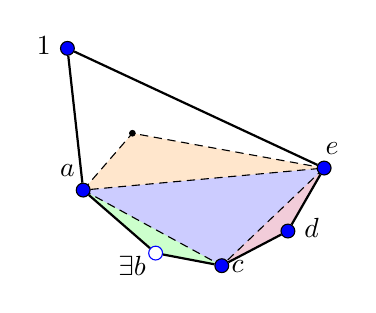
\begin{tikzpicture}
           
        % \node[draw, circle, black, fill=black, inner sep=0pt, minimum size=2pt] (p2) at (2.5,0.67*1.4) {};
        % \node[draw, circle, black, fill=black, inner sep=0pt, minimum size=2pt] (p3) at (1.4,-0.1) {};
    
    
        \coordinate (a) at (0,0.4);
        \coordinate (b) at (0.92*1,-0.5*0.8);
        \coordinate (c) at (1.6*1.1, -0.7*0.8);
        \coordinate (d) at (2.6*1,-0.3*0.4);
        \coordinate (e) at (1.8*1.7,0.4*1.7);

        \coordinate (p1) at (0.25*2.5, 0.66*1.7);
        \coordinate (p2) at (2.5,0.67*1.4);
        \coordinate (p3) at (1.4,-0.1);

        \fill[blue, opacity=0.2] (a) -- (c) -- (e) -- cycle;
         \fill[orange, opacity=0.2] (a) -- (p1) -- (e) -- cycle;
        \fill[purple, opacity=0.2] (c) -- (d) -- (e) -- cycle;
        \fill[green, opacity=0.2] (a) -- (b) -- (c) -- cycle;
        % \draw[densely dashed] (a) -- (c) -- (e) -- (a);


         \draw[densely dashed] (a) -- (c) -- (e) -- (a);

       
        \draw[densely dashed] (a) -- (p1) -- (e);

        \node[draw, circle, black, fill=blue, inner sep=0pt, minimum size=5pt,label={[xshift=-0.2cm, yshift=-0.05cm]$a$}] (a) at (0,0.4) {};
        \node[draw, circle, blue,  fill=white, inner sep=0pt, minimum size=5pt, label={[xshift=-0.3cm, yshift=-0.5cm]$\exists b$}] (b) at (0.92*1,-0.5*0.8) {};
        \node[draw, circle, black, fill=blue, inner sep=0pt, minimum size=5pt, label={[xshift=0.2cm, yshift=-0.3cm]$c$}] (c) at (1.6*1.1, -0.7*0.8) {};
        \node[draw, circle, black, fill=blue, inner sep=0pt, minimum size=5pt, label={[xshift=0.3cm, yshift=-0.3cm]$d$}] (d) at (2.6*1,-0.3*0.4) {};
        \node[draw, circle, black, fill=blue, inner sep=0pt, minimum size=5pt, label={[xshift=-0.3cm, yshift=-0.3cm]$1$}] (1) at (-0.2*1,2.2) {};
        

    % \node[draw, circle, black, fill=blue, inner sep=0pt, minimum size=5pt,label={[xshift=-0.1cm, yshift=-0.05cm]$a$}] (a) at (0,0) {};
    % \node[draw, circle, blue,  inner sep=0pt, minimum size=5pt, label={[xshift=-0.1cm, yshift=-0.05cm]$\exists b$}] (b) at (0.3*1.5,0.6*1.9) {};
    % \node[draw, circle, blue, inner sep=0pt, minimum size=5pt, label={[xshift=-0.1cm, yshift=-0.05cm]$\exists c$}] (c) at (0.8*1.7, 0.9*1.7) {};
    % \node[draw, circle, black, fill=blue, inner sep=0pt, minimum size=5pt, label={[xshift=0.1cm, yshift=-0.05cm]$d$}] (d) at (1.3*1.9,0.7*1.8) {};
    \node[draw, circle, black, fill=blue, inner sep=0pt, minimum size=5pt, label={[xshift=0.1cm, yshift=-0.05cm]$e$}] (e) at (1.8*1.7,0.4*1.7) {};
    % \node[draw, circle, black, fill=blue, inner sep=0pt, minimum size=5pt, label={[xshift=0.4cm, yshift=-0.4cm]$f$}] (f) at (0.9*1.7,-0.2*1.7) {};
    % \draw[thick] (a) -- (b) -- (c) -- (d) -- (e) -- (f) -- (a);

 \node[draw, circle, black, fill=black, inner sep=0pt, minimum size=2pt] (p1) at (0.25*2.5,0.66*1.7) {};
 \draw[thick] (1) -- (a) -- (b) -- (c) -- (d) -- (e) -- (1);
        % \draw[densely dashed] (c) -- (p2) -- (e);
        \end{tikzpicture}
        \caption{$(\vvar_{a,c,d} \land \orvar_{c, d, e} \land \hvar_{a,c,e})$}\label{fig:clause-15-forbid}
    \end{subfigure}
    \caption{Illustration of some \emph{forbidden configurations} that imply $6$-holes. \Cref{fig:clause-13-forbid} corresponds to the configuration forbidden by~\Cref{eq:no6Hole1Below}, \Cref{sub@fig:clause-14-forbid} to the one forbidden by~\Cref{eq:no6Hole2Below1}, and~\Cref{fig:clause-15-forbid} to~\Cref{eq:no6Hole3Below}. All highlighted regions correspond to empty triangles.}\label{fig:forbidden}
\end{figure}


\subparagraph*{Satisfaction.}
We now have to justify that the clauses of $\phi_n$
are satisfied by the intended interpretation $\tau_S$
for a $6$-hole-free point set $S$.
The variable-defining clauses~\labelcref{eq:insideClauses1,eq:insideClauses2,eq:holeDefClauses1,eq:capDef,eq:cupDef,eq:capFDef,eq:capDef2,eq:cupDef2}
follow essentially by definition combined with boolean reasoning.
The orientation properties~\labelcref{eq:signotopeClauses11,eq:signotopeClauses12}
have been established in the family of theorems \lstinline|σ_propᵢ|.
The lexicographic ordering clauses~\labelcref{eq:revLexClauses}
follow from the \textbf{Lex order} property of canonical positions.
Thus we are left with clauses~\labelcref{eq:no6Hole1Below,eq:no6Hole4Above,eq:no6Hole2Below1,eq:no6Hole2Below2,eq:no6Hole3Below}
which forbid the presence of certain $6$-holes.\footnote{
They are intended to forbid \emph{all} $6$-holes,
but proving completeness is not necessary for an unsatisfiability-based result.}
We illustrate why clause~\labelcref{eq:no6Hole1Below} is true.
The contrapositive is easier to state:
if $\tau_S$ satisfies $\ufvar_{a,d,e}\wedge\orvar_{a,p,e}$,
then $S$ contains a $6$-hole.
The intuitive argument is depicted in~\Cref{fig:clause-13-forbid}.
The clause directly implies the existence of a convex hexagon $apedcb$
such that $ace$ is a $3$-hole.
It turns out that this is enough to ensure
the existence of a $6$-hole by ``flattening'' the triangles $ape$, $edc$, and $cba$,
if necessary,
to obtain empty triangles $ap'e$, $ed'c$, and $cb'a$,
which can be assembled into a $6$-hole $ap'ed'cb'$.

Justifying this formally turned out to be complex,
requiring a fair bit of reasoning about point \lstinline|Arc|s
and \lstinline|σCCWPoints|: lists of points winding around a convex polygon.
Luckily, the main argument can be summarized in terms of two facts:
(a) any triangle $abc$ contains an empty triangle $ab'c$; and
(b) empty shapes sharing a common line segment can be glued together.
Formally, (a) can be stated as

\begin{lstlisting}
theorem σIsEmptyTriangleFor_exists (gp : ListInGenPos S)
  (abc : [a, b, c] ⊆ S) : ∃ b' ∈ S, σ a b' c = σ a b c
    ∧ (b' = b ∨ σPtInTriangle b' a b c) ∧ σIsEmptyTriangleFor a b' c S.toFinset
\end{lstlisting}
\begin{proof}
  Given points $p,q$, say that $p \leq q$ iff $p$ is in the triangle $aqc$.
  This is a preorder.
  Now, the set $S' = \{x \in S \mid \sigma(a,x,c) = \sigma(a,b,c) \wedge x \leq b\}$
  is finite and so has a weakly minimal element $b'$,
  in the sense that no $x \in S'$ has $x < b'$.
  Emptiness of $ab'c$ follows by minimality.
\end{proof}

Moving on, (b) follows from a \emph{triangulation lemma}:
given any convex point set $S$
and a line $\overleftrightarrow{ab}$ between two vertices of $S$,
the convex hull of $S$ is contained in the convex hulls
of points on either side of $\overleftrightarrow{ab}$.
That is:
\begin{lstlisting}
theorem split_convexHull (cvx : ConvexIndep S) :
  ∀ {a b}, a ∈ S → b ∈ S →
    convexHull ℝ S ⊆ convexHull ℝ {x ∈ S | σ a b x ≠ ccw}
                    ∪ convexHull ℝ {x ∈ S | σ a b x ≠ cw}
\end{lstlisting}
\begin{figure}
    \centering
    \begin{subfigure}{0.45\textwidth}
        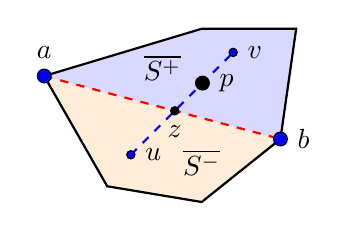
\begin{tikzpicture}
        \coordinate (a) at (0, 0.4);
        \coordinate (b) at (3, -0.4);
        \coordinate (v1) at (3.2, 1);
        \coordinate (v2) at (2, 1);
        \coordinate (u1) at (0.8, -1);
        \coordinate (u2) at (2, -1.2);
        \coordinate (u) at (1.1, -0.6);
        \coordinate (v) at (2.4, 0.7);
        \coordinate (p) at (2.01,0.31);
        \coordinate (z) at (1.65789, -0.0421053);

        \fill[blue, opacity=0.15] (b) -- (v1) -- (v2) -- (a) -- cycle;
        \fill[orange, opacity=0.15] (a) -- (u1) -- (u2) -- (b) -- cycle;

        \draw[thick] (a) -- (u1) -- (u2) -- (b) -- (v1) -- (v2) -- (a);
        \draw[dashed, thick, red] (a) -- (b);
        \draw[dashed, thick, blue] (u) -- (v);

        \node[draw, circle, black, fill=blue, inner sep=0pt, minimum size=5pt, label=above:$a$] (pA) at (a) {};
        \node[draw, circle, black, fill=blue, inner sep=0pt, minimum size=5pt, label=right:$b$] (pB) at (b) {};
        \node[draw, circle, black, fill=blue, inner sep=0pt, minimum size=3pt, label=right:$u$] (pU) at (u) {};
        \node[draw, circle, black, fill=blue, inner sep=0pt, minimum size=3pt, label=right:$v$] (pV) at (v) {};

        \node[draw, circle, black, fill=black, inner sep=0pt, minimum size=5pt, label=right:$p$] (pP) at (p) {};
        \node[draw, circle, black, fill=black, inner sep=0pt, minimum size=3pt, label=below:$z$] (pZ) at (z) {};

        \node[] at (1.5, 0.5) {$\overline{S^+}$};
        \node[] at (2, -0.7) {$\overline{S^-}$};

        \end{tikzpicture}
        \caption{}\label{fig:triangulation2-a}
    \end{subfigure}
    \begin{subfigure}{0.45\textwidth}
        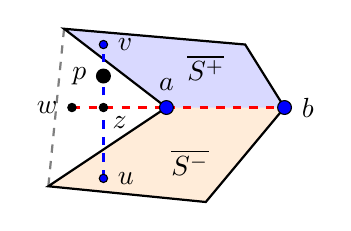
\begin{tikzpicture}
            \coordinate (a) at (1.5, 0);
            \coordinate (b) at (3, 0);
            \coordinate (v1) at (2.5, 0.8);
            \coordinate (v2) at (0.2, 1);
            \coordinate (u1) at (0, -1);
            \coordinate (u2) at (2, -1.2);
            \coordinate (u) at (0.7, -0.9);
            \coordinate (v) at (0.7, 0.8);
            \coordinate (p) at (0.7, 0.4);
            \coordinate (z) at (0.7, 0);
            \coordinate (w) at (0.3, 0);

            \fill[blue, opacity=0.15] (b) -- (v1) -- (v2) -- (a) -- cycle;
            \fill[orange, opacity=0.15] (a) -- (u1) -- (u2) -- (b) -- cycle;

            \draw[thick] (a) -- (u1) -- (u2) -- (b) -- (v1) -- (v2) -- (a);
            \draw[dashed, thick, red] (a) -- (b);
            \draw[dashed, thick, blue] (u) -- (v);
            \draw[dashed, thick, red] (w) -- (a);
            \draw[dashed, thick, opacity=0.5] (v2) -- (u1);

            \node[draw, circle, black, fill=blue, inner sep=0pt, minimum size=5pt, label=above:$a$] (pA) at (a) {};
            \node[draw, circle, black, fill=blue, inner sep=0pt, minimum size=5pt, label=right:$b$] (pB) at (b) {};
            \node[draw, circle, black, fill=blue, inner sep=0pt, minimum size=3pt, label=right:$u$] (pU) at (u) {};
            \node[draw, circle, black, fill=blue, inner sep=0pt, minimum size=3pt, label=right:$v$] (pV) at (v) {};

            \node[draw, circle, black, fill=black, inner sep=0pt, minimum size=5pt, label=left:$p$] (pP) at (p) {};
            \node[draw, circle, black, fill=black, inner sep=0pt, minimum size=3pt, label={[shift={(-0.05,0.05)}]-45:$z$}] (pZ) at (z) {};
            \node[draw, circle, black, fill=black, inner sep=0pt, minimum size=3pt, label=left:$w$] (pW) at (w) {};

            \node[] at (2, 0.5) {$\overline{S^+}$};
            \node[] at (1.8, -0.7) {$\overline{S^-}$};

        \end{tikzpicture}
        \caption{}\label{fig:triangulation2-b}
    \end{subfigure}
    \caption{Illustration of the proof for \lstinline|split_convexHull|. (a) Given point $p$, we obtain points $u$ and $v$ inside the two halves and $z$ as the point of intersection with the line $\overline{ab}$. (b) In this (contradictory) situation, the point $z$ has ended up outside the segment $\overline{ab}$, because $S$ is not actually convex. In this case we construct $w$ such that $z$ is on the $\overline{wa}$ segment, and observe that $w,z,a,b$ are collinear.}\label{fig:triangulation2}
\end{figure}

\begin{proof}
    Let $S^+=\{x\in S\mid \sigma(a,b,x)\ge 0\}$ and $S^-=\{x\in S\mid \sigma(a,b,x)\le 0\}$ be the two sets in the theorem, and let $p\in \overline{S}$, where $\overline{S}$ denotes the convex hull of $S$. Assume WLOG that $\sigma(a,b,p)\ge 0$. (We would like to show that $p\in \overline{S^+}$.) Now $p$ is a convex combination of elements of $S^+$ and elements of $S^-$, so there exist points $u\in \overline{S^-}$ and $v\in \overline{S^+}$ such that $p$ lies on the $\overline{uv}$ line.
%
    Because $\{x\mid \det(a,b,x)\le 0\}\supseteq S^-$ is convex, it follows that $\det(a,b,u)\le 0$, and likewise $\det(a,b,v)\ge 0$, so they lie on opposite sides of the $\overleftrightarrow{ab}$ line and hence $\overline{uv}$ intersects $\overleftrightarrow{ab}$ at a point $z$. The key point is that $z$ must in fact be on the line segment $\overline{ab}$; assuming that this was the case, we could obtain $z$ as a convex combination of $a$ and $b$, and $p$ as a convex combination of $v$ and $z$, and since $v$ is in $\overline{S^+}$ and $a,b\in S^+\subseteq\overline{S^+}$ we can conclude $p\in \overline{S^+}$.
%
    To show that $z\in \overline{ab}$, suppose not, so that $a$ lies between $z$ and $b$ (see \Cref{fig:triangulation2-b}). (The case where $z$ is on the $b$ side is similar.) We can decompose $z$ as a convex combination of some $w\in \overline{S\setminus\{a\}}$ and $a$, which means that $w,z,a,b$ are collinear and appear in this order on the line. Therefore $a$ is a convex combination of $w$ and $b$, which means that $a\in \overline{S\setminus\{a\}}$ which violates convexity of $S$.
\end{proof}

\noindent
By contraposition,
the triangulation lemma directly implies that
if $\{x \in S \mid \sigma(a,b,x) \neq +1\}$ and $\{x \in S \mid \sigma(a,b,x) \neq -1\}$
are both empty shapes in $P$,
then $S$ is an empty shape in $P$.

\subsection{Running the CNF.}
\label{sec:running_cnf}
Having now shown that our main result follows if $\phi_{30}$ is unsatisfiable,
we run a distributed computation to check its unsatisfiability.
We solve the SAT formula~$\phi_{30}$ produced by Lean using the same setup as
Heule and Scheucher~\cite{emptyHexagonNumber}, although using different hardware:
the Bridges 2 cluster of the Pittsburgh Supercomputing Center~\cite{cluster}.
Following Heule and Scheucher,
we partition the problem into 312\,418 subproblems.
Each of these subproblems was
solved using {\tt CaDiCaL} version 1.9.5.
{\tt CaDiCaL} produced an LRAT proof for each execution,
which was validated using the {\tt cake\_lpr} verified checker on-the-fly
in order to avoid writing/storing/reading large files.
The total runtime was 25\,876.5 CPU hours, or roughly 3 CPU years.
The difference in runtime relative to Heule and Scheucher's original run
is purely due to the difference in hardware.
Additionally,
we validated that the subproblems cover the entire search space
as Heule and Scheucher did~\cite[Section 7.3]{emptyHexagonNumber}.
This was done by verifying the unsatisfiability
of another formula that took 20 seconds to solve.

The artifact for this paper includes scripts to validate any individual subproblem,
as well as the summary proof that the subproblems cover the search space.
However, the unsatisfiability of $\phi_{30}$ depends on
the unsatisfiability of \textit{all} (hundreds of thousands of) subproblems.
A skeptical reader might wish to examine the proof files for all subproblems,
but we estimated the total proof size to be tens or hundreds of terabytes,
far too much to reasonably store and distribute.
Instead, the skeptical reader must run the entire 3 CPU year computation.
We believe this trust story can be somewhat improved,
but we leave such a challenge to future work.

% file-local attic:

% By using the triangulation lemma repeatedly,
% we can slice up a convex $k$-gon into smaller pieces in any way we like until we get to triangles,
% thereby showing that convex polygons can be triangulated.


% \section{SAT Pipeline}\label{sec:leansat}
% This section describes the bridge between mathematical objects and the propositional variables representing them in the context of a CNF formula.
Consider the following theorem:

\begin{lstlisting}
theorem EmptyTriangle10TheoremLists
    (pts : List Point) (gp : PtListInGP pts) (h : pts.length = 10) :
    HasEmptyTriangle pts.toFinset
\end{lstlisting}

% We wish to prove that no list of $10$ points in general position can avoid an empty triangle.
% Consider the propositional formula $\varphi$ over variables $\orvar_{p, q, r}$, with $1 \leq p  < q < r \leq 10$.
% \begin{enumerate}
%     % \item $\left(\neg \orvar_{p, q, r} \lor \neg \orvar_{p, r, t} \lor \orvar_{p, q, t}\right) \land \left(\orvar_{p, q, r} \lor \orvar_{p, r, t} \lor  \neg \orvar_{p, q, t}\right)$
%     % &\left(\neg \orvar_{p, q, r} \lor \neg \orvar_{q, r, t} \lor  \orvar_{p, r, t}\right) \land \left(\orvar_{p, q, r} \lor \orvar_{q, r, t} \lor  \neg \orvar_{p, r, t}\right).
% \end{enumerate}





% Describe how we go from abstract formula over boolean variables
% to a CNF using encoding programs.
% CNF is usually large, and SAT solvers take the CNF in a format called DIMACS which is not human inspectable.
% Thus usually generated by encoding program rather than constructed manually.
% This DIMACS is fed to a SAT solver, which produces an UNSAT certificate
% (usually in a format known as DRAT or LRAT).

% Given this pipeline, we have two distinct concerns for correctness:
% \begin{itemize}
%     \item[(1)] \textbf{Is the CNF formula correct?}
%     We want to formally verify that our ``encoder'' program
%     generates DIMACS output which
%     correctly represent the abstract formula we wish to show UNSAT.
%     \item[(2)] \textbf{Is the SAT solver output correct?}
%     The UNSAT certificate must be checked for correctness
%     against the DIMACS formula.
% \end{itemize}

% Prior work on (2) has produced highly trustworthy proof checkers
% for SAT solver output (cake lpr citation, GRAT citation maybe?).
% We rely on \texttt{cake\_lpr} for this step of the proof,
% and trust that the DIMACS formula given to \texttt{cake\_lpr}
% is unsatisfiable if this program terminates without error.

% In contrast, we found very little prior work on (1).
% Codel (cite Codel, any other papers Cayden found about this).

% We built on (bryant citation, codel citation)
% to develop tools for writing correct-by-construction encoding programs
% against an abstract model of propositional formulas.
% This infrastructure is a component of the fledgling \leansat{} library,
% which is largely outside the scope of this paper.
% Nonetheless this library enabled us to re-implement
% Heule et al's encoding exactly as presented (TODO: is this true?).

% Here we give a brief overview of how this section of the formalization proceeds.

% \subsection{Variables}

% The \leansat{} library allows formulas to be written over arbitrary variable sets.
% As an example, for the Empty Triangle Theorem (see section 5) we use the following variables:
% \begin{lstlisting}
% inductive Var (n : Nat)
%   | sigma  (a b c : Fin n)
%   | inside (x a b c : Fin n)
%   | hole   (a b c : Fin n)
% \end{lstlisting}
% TODO explain how the library handles converting these variables to \(\mathbb{N}\)
% for the purposes of DIMACS.

% \subsection{Abstract Propositional Formula}

% Given that the encoding presented in Heule et al has many sets of clauses,
% we divide the abstract formula into a few sub-formulas.
% Here is the formula which defines the "is hole" variables:
% \begin{lstlisting}
% /--
%   Triangle abc is a hole iff all x are not inside triangle abc.
% -/
% def holeDefs (n : Nat) : PropAssignment (Var n) → Prop := fun τ =>
%   ∀ {a b c}, τ (Var.hole a b c) ↔
%     (∀ x, a < x → x < c → x ≠ b →
%       !τ (Var.inside x a b c))
% \end{lstlisting}
% The Lean statement here is clean and simple,
% and nicely corresponds to the paper presentation.
% We define the entire formula in around 100 lines of Lean.
% TODO(JG): get exact numbers

% \subsection{Encoding Program}

% Now that we have defined an abstract formula over our variables,
% we need to write a program which encodes this formula to DIMACS.
% Again we divide the program into sub-programs,
% corresponding exactly to how we divided up the formula.
% Here is the signature of the encoder for the formula from the previous section:
% \begin{lstlisting}
% def holeDefClauses (n : Nat) : VEncCNF (Var n) Unit (holeDefs n) :=
%   ...
% \end{lstlisting}
% The \texttt{VEncCNF} type is essentially a state monad,
% where the state is the DIMACS output.
% However, it is constrained to those programs which
% verifiably encode the predicate \texttt{holeDefs n}.

% In particular, if we run \texttt{holeDefClauses n},
% we get DIMACS output which is satisfiable iff \texttt{holeDefs n} is satisfiable,
% no matter what the particulars are in \texttt{holeDefClauses}.
% This is expressed in the following theorem from \leansat{}:
% \begin{lstlisting}
% theorem toICnf_equisatisfiable [FinEnum ν] (v : VEncCNF L α P) :
%   (∃ τ : PropAssignment IVar, τ |= v.val.toICnf.toPropFun) ↔
%     (∃ τ : PropAssignment ν, P τ)
% \end{lstlisting}
% TODO(JG): cleanup in leansat

% The encoding program, and its verification,
% takes a few hundred lines of Lean.
% TODO(JG) update when done rewriting

% \subsection{Verifying UNSAT Proof}

% We have generated a DIMACS-format formula which is satisfiable iff
% our abstract encoding is satisfiable.
% Ideally, at this point we would emit the formula,
% run a SAT solver,
% get a proof of unsatisfiability,
% and then check this proof \textit{in the trusted Lean kernel}.
% This approach would establish the formula unsatisfiable
% with the same level of trust as all mathematics verified in Lean.

% Unfortunately, such an approach is not feasible due to performance constraints.
% The Lean kernel is simple and trustworthy,
% but evaluates programs quite slowly,
% orders of magnitude slower than executing compiled Lean programs.
% The \(h(6) = 30\) result generated on the order of 100 TB of DRAT proof,
% which is far, far beyond the range at which the kernel could feasibly check.

% TODO(JG): explain our new trust story for this last leg of the journey.

% \begin{lstlisting}
% axiom cnfUnsat : ¬∃ τ, τ |= (theEncoding 30).toICNF
% \end{lstlisting}
% TODO(JG): make this statement reality


\section{Related Work}\label{sec:related-work}
Our formalization is closely related to a prior development
in which Marić put proofs of $g(6) \leq 17$ on a more solid foundation \cite{19maric_fast_formal_proof_erdos_szekeres_conjecture_convex_polygons_most_six_points}.
The inequality,
originally obtained by Szekeres and Peters \cite{06szekeres_computer_solution_17_point_erdos_szekeres_problem}
using a bespoke, unverified search algorithm,
was confirmed in the work of Marić
by means of a formally verified SAT encoding.
Introducing an optimized encoding based on nested convex hull structures
and leveraging accumulated progress in SAT solving technology [citation?],
this approach also improved on the time to solution

Our work focuses on the closely related problem
of determining $k$-hole numbers $h(k)$.
Rather than devising a new SAT encoding,
we use one from Heule and Scheucher \cite{emptyHexagonNumber}
in a lightly modified form.

Despite the different focus,
a proof of $g(6) \leq 17$ can be obtained easily
as a corollary of our development:
asserting the hole variables $\hvar_{a,b,c}$ as unit clauses,
leaving the remainder of the encoding in~\Cref{fig:full-encoding} unchanged,
trivializes constraints that have to do with emptiness
so that only convexity constraints remain.
The resulting CNF formula
asserts the existence of a set of $n$ points
with no convex $6$-gon.
We find this formula to be unsatisfiable for $n = 17$,
giving the classic
\begin{lstlisting}
theorem gon_6_theorem (pts : List Point) (gp : Point.ListInGenPos pts)
    (h : pts.length ≥ 17) : HasConvexKGon 6 pts.toFinset
\end{lstlisting}
However, it would not be as easy
to attack $g(k)$ for $k \neq 6$ using this particular encoding.

As both formalizations are executable,
we can perform a direct comparison against Marić's encoding.
On a personal laptop,
we find that it takes negligible time (below 1s)
for our verified Lean encoder to generate a CNF,
which then takes around 28s to solve.
In contrast,
the Isabelle/HOL-based encoder takes around 10 minutes [TODO precis] to generate a CNF,
which then takes around 787s to solve.

To avoid encoding overhead,
Marić resorts to trusting a C++ encoder
whose code has been manually compared against the Isabelle/HOL specification:
something we do not have to do.
The difference in solving time
can likely be accounted for by differences in the respective encodings,
in particular their symmetry breaking strategies.
The encoding of Heule and Scheucher uses $\mathcal O(n^4)$ clauses
to look for a $6$-hole or $6$-gon in $n$ points,
whereas the one of Marić uses $\mathcal O(n^6)$ clauses.
They are based on different ideas:
the former as detailed in~\Cref{sec:symmetry-breaking},
whereas the latter on nested convex hulls.
The different approaches have been discussed by Scheucher \cite{scheucherTwoDisjoint5holes2020}.
The progress in solving times
represents an encouraging state of affairs;
we are optimistic that if continued,
it could lead to an eventual resolution of $g(7)$.

Further differences regard what exactly was formally proven.
Like most work in this area,
we use the combinatorial abstraction of triple orientations.
We and Marić alike show that point sets in $\mathbb R^2$
satisfy orientation properties (\Cref{sec:properties-of-sigma}).
However, our work goes further in building the connection
between geometry and combinatorics:
our definitions of convexity and emptiness (\Cref{sec:geometry}),
and consequently the theorem statements,
are the geometric ones based on convex hulls
as defined in Lean's \texttt{mathlib} \cite{20lean_mathematical_library}.
In contrast, Marić axiomatizes these as being about specific values of $\sigma$.
Thus one has to trust that each combinatorial abstraction
corresponds exactly to the geometric concept.

A final point of difference concerns the verification of SAT proofs.
Marić fully reconstructs some of their results,
though not the main one for $g(6)$,
in an NbE-based proof checker for Isabelle/HOL.
We make no such attempt for the time being,
instead passing our SAT proofs through the the formally verified proof checker \texttt{cake\_lpr} \cite{tanVerifiedPropagationRedundancy2023}
and asserting unsatisfiability of the CNF as an axiom in Lean.
Thus we are trusting that the CNF formula produced by the verified Lean encoder
is the same one whose unsatisfiability was checked by \texttt{cake\_lpr}.
Everything else has been verified.

We know of no other formal proofs of Erd\H{o}s-Szekeres-type problems.

% WN: Maybe put this in the symmetry breaking section?
Compared to the work of Heule and Scheucher which we have verified \cite{emptyHexagonNumber},
besides the significant improvement in trust,
we have streamlined the symmetry breaking argument somewhat.
It no longer requires applying continuity of the determinant map,
or shearing points to have positive $y$ coordinates.

% WN: Anything else that should be mentioned here?


\section{Concluding Remarks}\label{sec:conclusions}
This formalization required approximately 300 hours of work over 3 months
by researchers with significant experience formalizing mathematics in Lean.
The final version of our proofs consists of approximately 4.7k lines of Lean code
(including comments/whitespace);
about $26\%$ consists of lemmas that should be moved to upstream libraries,
about $40\%$ develops the mathematical theory of orientations in plane geometry,
and the remaining $34\%$ (1550 LOC) validates the symmetry breaking and SAT encoding.
Many more lines of code were deleted or rewritten,
so these numbers should be taken with a grain of salt.

We substantially simplified the symmetry-breaking argument presented by Heule and Scheucher.
Beyond that, though, the correctness argument remains generally the same.
So what did formal verification contribute in this case?

We have substantially improved the level of trust in the new result by Heule and Scheucher.
Prior to formalization,
their result relied on the correctness of various components that are hard to validate manually,
while now we can assert with high confidence that their result is correct.
Beyond the main theorem presented here,
we demonstrated our approach for formalizing reductions to UNSAT,
and developed a broadly useful formal theory of orientations and plane geometry.

\subparagraph*{Future work.}
The geometric and combinatorial machinery developed for this formalization
will be useful in future formalizations of Erd\H{o}s-Szekeres style problems.
We believe automated reasoning will continue to be used in this area,
and hope future results can be verified with much less effort.
Beyond automated reasoning,
we hope to see formalizations of traditional pen and paper proofs in this area,
perhaps starting with a (formal) proof of the lower bound for the $h(6) = 30$ result.

We also believe work should be done towards improving the connection between verified SAT tools and ITPs.
Although we are confident that our results are correct,
the trust story at the connection point clearly has room for improvement,
starting with some simple automation for running verified SAT toolchains from Lean.


\bibliography{main}

\end{document}

